\documentclass[
size=10pt,
paper=screen,
mode=present,
display=slidesnotes,
style=uwr,
nohandoutpagebreaks,
%pauseslide,
fleqn,
clock,
%,draft
]{powerdot}

\usepackage[utf8]{inputenc}
%\usepackage{polski}
\usepackage[english]{babel}
\usepackage{pstricks}
\usepackage{color}
\usepackage{xcolor}
\usepackage{tcolorbox}
\usepackage{import}
\usepackage{pstricks-add}
\usepackage{pst-grad}
\usepackage{pst-text}
\usepackage{pst-coil}
\usepackage{pst-node}
\usepackage{pst-plot}
\usepackage{array}
\usepackage{amsmath}
\usepackage{amssymb}
\usepackage{multirow}
\usepackage{graphicx}
\usepackage{verbatim}
\usepackage{fancyvrb}
\usepackage{hyperref}
\hypersetup{colorlinks=true, urlcolor=pdcolor4}
\usepackage{tikz}
\usepackage{tikz-3dplot}
\usetikzlibrary{positioning,arrows,fadings,decorations.pathreplacing,decorations.pathmorphing,decorations.markings,shapes,backgrounds,snakes}
\tikzstyle{common} = [draw, ultra thick, text centered, inner sep = 0pt, outer sep = 0pt]

\tikzstyle{filled}[pdcolor1]    = [common, color = pdcolor2, fill = #1]
\tikzstyle{filled2}[pdcolor1]    = [common, color = #1, fill = #1]
\tikzstyle{notFilled}[pdcolor1] = [common, color = #1, fill = pdcolor2]

\tikzstyle{line}[pdcolor1] = [>=latex, color = #1, shorten <= 2pt, shorten >= 2pt]
\tikzstyle{curl}[pdcolor1] = [color = #1, snake = coil, segment length = 5pt, line after snake = 0pt, line before snake = 0pt, segment aspect = 0]

\tikzstyle{round} = [rounded corners = 5pt]

\tikzstyle{rectS}  = [rectangle, minimum width = 1.75cm, text width = 1.75cm, minimum height = 0.75cm]
\tikzstyle{rect}  = [rectangle, minimum width = 2.5cm, text width = 2.5cm, minimum height = 1cm]
\tikzstyle{rectH} = [rectangle, minimum width = 0.5cm, text width = 0.5cm, minimum height = 2cm]
\tikzstyle{ell}  = [ellipse, minimum height = 1cm, minimum width = 2.5cm]
\tikzstyle{diam} = [diamond, minimum height = 1cm, minimum width = 2.5cm]
\tikzstyle{circ}  = [ellipse, minimum height = 1.5cm, minimum width = 1.5cm]

\usepackage{ifthen}
\usepackage{pgfplots}
\usepackage{soul}
\usepackage{hyperref}
\usepackage{enumitem}

\setlist[itemize]{itemsep=10pt}

\renewcommand\Re{\operatorname{Re}}
\renewcommand\Im{\operatorname{Im}}

\setlength{\fboxsep}{2pt}
\setlength{\fboxrule}{0pt}

\newcommand{\myBox}[2][pdcolor1]{\begin{center}\colorbox{#1}{\framebox[0.75\columnwidth][c]{\parbox{0.7\columnwidth}{\color{pdcolor2}\textnormal{#2}}}}\end{center}}
\newcommand{\myBoxFullWidth}[2][pdcolor1]{\begin{center}\colorbox{#1}{\framebox[\columnwidth][c]{\parbox{0.95\columnwidth}{\color{pdcolor2}\textnormal{#2}}}}\end{center}}
\newcommand{\myFrame}[2][pdcolor1]{\begin{center}\fboxrule=1pt\fboxsep=5pt\colorbox{pdcolor2}{\framebox[0.78\columnwidth][c]{\parbox{0.7\columnwidth}{\color{#1}\textnormal{#2}}}}\end{center}}
\newcommand{\myFrameFullWidth}[2][pdcolor1]{\begin{center}\fboxrule=1pt\fboxsep=5pt\colorbox{pdcolor2}{\framebox[\columnwidth][c]{\parbox{0.95\columnwidth}{\color{#1}\textnormal{#2}}}}\end{center}}
\newcommand{\myFrameTextWidth}[2][pdcolor1]{\begin{center}\fboxrule=1pt\colorbox{pdcolor2}{\framebox[0.9\textwidth][c]{\color{#1}\textnormal{#2}}}\end{center}}


\newcommand{\sep}{\mbox{}\\}

\makeatletter
\@addtoreset{footnote}{page}
\renewcommand\@makefnmark{\hbox{\@textsuperscript{\normalfont\color{pdcolor4}\@thefnmark}}}
\makeatother

\renewcommand{\thefootnote}{\ifcase\value{footnote}\or *\or **\or ***\or ****\fi}

\renewcommand{\black}[1]{\color{pdcolor1}{#1}}
\renewcommand{\white}[1]{\color{pdcolor2}{#1}}
\newcommand{\grey}[1]{\color{pdcolor3}{#1}}
\renewcommand{\green}[1]{\color{pdcolor4}{#1}}
\newcommand{\orange}[1]{\color{pdcolor5}{#1}}
\renewcommand{\red}[1]{\color{pdcolor6}{#1}}
\renewcommand{\blue}[1]{\color{pdcolor7}{#1}}
\renewcommand{\yellow}[1]{\color{pdcolor8}{#1}}



\pdsetup{
  lf = Tomasz Golan,
  cf = NuWro @ HEP UW
}

\title{NuWro - neutrino MC event generator}
\author{Tomasz Golan}
\date{28.04.2017, UW HEP Seminar}

\begin{document}

\maketitle

%\section{Introduction}

%%%%% NEUTRINO PROPERTIES %%%%%

\begin{slide}[toc=Neutrino properties]{Basic properties of neutrinos}
  
  % elementary particles table
  \rput(0.8\slidewidth,0.0\slideheight){\scalebox{0.75}{% elementary particles table
\begin{pspicture}

  \psframe[linestyle = none, fillstyle = solid, fillcolor = pdcolor3](3,4)(3.8,4.8)\rput[c](3.4,4.4){\color{pdcolor2} $H$}

  \psframe[shadow = true, shadowsize = 0.05, shadowcolor = pdcolor3, linewidth = 0.01, linecolor = pdcolor1](0,3)(.8,3.8)\rput[c](0.4,3.4){\color{pdcolor1} $u$}
  \psframe[shadow = true, shadowsize = 0.05, shadowcolor = pdcolor3, linewidth = 0.01, linecolor = pdcolor1](1,3)(1.8,3.8)\rput[c](1.4,3.4){\color{pdcolor1} $c$}
  \psframe[shadow = true, shadowsize = 0.05, shadowcolor = pdcolor3, linewidth = 0.01, linecolor = pdcolor1](2,3)(2.8,3.8)\rput[c](2.4,3.4){\color{pdcolor1} $t$}
  \psframe[linestyle = none, fillstyle = solid, fillcolor = pdcolor1](3,3)(3.8,3.8)\rput[c](3.4,3.4){\color{pdcolor2} $\gamma$}
  
  \psframe[shadow = true, shadowsize = 0.05, shadowcolor = pdcolor3, linewidth = 0.01, linecolor = pdcolor1](0,2)(.8,2.8)\rput[c](0.4,2.4){\color{pdcolor1} $d$}
  \psframe[shadow = true, shadowsize = 0.05, shadowcolor = pdcolor3, linewidth = 0.01, linecolor = pdcolor1](1,2)(1.8,2.8)\rput[c](1.4,2.4){\color{pdcolor1} $s$}
  \psframe[shadow = true, shadowsize = 0.05, shadowcolor = pdcolor3, linewidth = 0.01, linecolor = pdcolor1](2,2)(2.8,2.8)\rput[c](2.4,2.4){\color{pdcolor1} $b$}
  \psframe[linestyle = none, fillstyle = solid, fillcolor = pdcolor1](3,2)(3.8,2.8)\rput[c](3.4,2.4){\color{pdcolor2} $g$}
  
  \psline[linewidth = 0.02, linestyle = dotted, linecolor = pdcolor1](0,1.875)(2.8,1.875)
  
  \psframe[shadow = true, shadowsize = 0.05, shadowcolor = pdcolor3, linewidth = 0.01, linecolor = pdcolor1](0,1)(.8,1.8)\rput[c](0.4,1.4){\color{pdcolor1} $\nu_e$}
  \psframe[shadow = true, shadowsize = 0.05, shadowcolor = pdcolor3, linewidth = 0.01, linecolor = pdcolor1](1,1)(1.8,1.8)\rput[c](1.4,1.4){\color{pdcolor1} $\nu_\mu$}
  \psframe[shadow = true, shadowsize = 0.05, shadowcolor = pdcolor3, linewidth = 0.01, linecolor = pdcolor1](2,1)(2.8,1.8)\rput[c](2.4,1.4){\color{pdcolor1} $\nu_\tau$}
  \psframe[linestyle = none, fillstyle = solid, fillcolor = pdcolor1](3,1)(3.8,1.8)\rput[c](3.4,1.4){\color{pdcolor2} $Z^0$}

  \psframe[shadow = true, shadowsize = 0.05, shadowcolor = pdcolor3, linewidth = 0.01, linecolor = pdcolor1](0,0)(.8,.8)\rput[c](0.4,0.4){\color{pdcolor1} $e$}
  \psframe[shadow = true, shadowsize = 0.05, shadowcolor = pdcolor3, linewidth = 0.01, linecolor = pdcolor1](1,0)(1.8,.8)\rput[c](1.4,0.4){\color{pdcolor1} $\mu$}
  \psframe[shadow = true, shadowsize = 0.05, shadowcolor = pdcolor3, linewidth = 0.01, linecolor = pdcolor1](2,0)(2.8,.8)\rput[c](2.4,0.4){\color{pdcolor1} $\tau$}
  \psframe[linestyle = none, fillstyle = solid, fillcolor = pdcolor1](3,0)(3.8,.8)\rput[c](3.4,0.4){\color{pdcolor2} $W^\pm$}
  
  \rput[c]{L}(-0.2,2.9){\footnotesize QUARKS}
  \rput[c]{L}(-0.2,0.9){\footnotesize LEPTONS}
  \rput[c]{R}(4, 1.9){\footnotesize BOSONS}
  \rput[c](1.4, 4.6){\scriptsize Three generations}
  \rput[c](1.4, 4.3){\scriptsize of fermions}
  \rput[c](0.4, 4){\footnotesize I}
  \rput[c](1.4, 4){\footnotesize II}
  \rput[c](2.4, 4){\footnotesize III}
  
\end{pspicture}
}}
  
  % neutrino oscillation
  \rput(0.15\slidewidth,-0.4\slideheight){\scalebox{0.5}{% neutrino oscillation
\begin{pspicture}
  
  \cnodeput[linestyle = none, fillstyle = solid, fillcolor = pdcolor1](0.5,0.57){nu1}{\Large\color{pdcolor2} $\nu_\alpha$}
    
  \psline[linewidth = 0.03, linecolor = pdcolor1](1.2, 0.57)(3.25, 0.57)
    
  \pscircle[linewidth = 0.03, linecolor = pdcolor1, linestyle = dotted](5, 0.57){1.75}
  \cnodeput[linestyle = none, fillstyle = solid, fillcolor = pdcolor7](5,1.7){nue}{\Large\color{pdcolor2} $\nu_e$}
  \cnodeput[linestyle = none, fillstyle = solid, fillcolor = pdcolor4](4,0){num}{\Large\color{pdcolor2} $\nu_\mu$}
  \cnodeput[linestyle = none, fillstyle = solid, fillcolor = pdcolor6](6,0){nut}{\Large\color{pdcolor2} $\nu_\tau$}

  \psline[linewidth = 0.03, linecolor = pdcolor1]{->}(6.75, 0.57)(8.8, 0.57)

  \cnodeput[linestyle = none, fillstyle = solid, fillcolor = pdcolor1](9.5,0.57){nu1}{\Large\color{pdcolor2} $\nu_\beta$}

  \psset{nodesep = 3pt}
  \ncarc[linecolor = pdcolor4]{->}{nue}{num}
  \ncarc[linecolor = pdcolor7]{->}{num}{nue}
  \ncarc[linecolor = pdcolor6]{->}{num}{nut}
  \ncarc[linecolor = pdcolor4]{->}{nut}{num}
  \ncarc[linecolor = pdcolor7]{->}{nut}{nue}
  \ncarc[linecolor = pdcolor6]{->}{nue}{nut}

\end{pspicture}
}}
  
  \vspace{-20pt}  
  \begin{itemize}

    \item $\frac{1}{2}$-spin, no electric charge, small mass \\ (extremely hard to detect)
    
    \item Interactions with elementary particles \\ $\rightarrow$ electroweak theory (Standard Model)
    
    \item Interactions with nucleons \\ $\rightarrow$ form factors \\ $\rightarrow$ parton distribution functions
    
    \item Interactions with nuclei $\rightarrow$ nuclear effects
        
    \item The neutrino flavor state is a superposition of the mass states: \\ \vspace{10pt}
    \hspace{160pt}$\left|\nu_\alpha\right> = \sum_i U_{\alpha i} \left|\nu_i\right>$
    \vspace{10pt}
    
    \hspace{125pt}The neutrino produced in $\alpha$ state \\ \hspace{125pt}can be measured in $\beta$ state.\\ \hspace{125pt}The phenomenon is called \\ \hspace{125pt}neutrino oscillation.
    
  \end{itemize}
    
\end{slide}

%%%%% PMNS MATRIX %%%%%

\begin{wideslide}[toc=PMNS matrix]{Pontecorvo-Maki-Nakagawa-Sakata matrix}
  
  The PMNS matrix defines the mass mixing in the lepton sector:
  
  $$U =    
    \left[\begin{array}{ccc}
      1 & 0 & 0 \\ 
      0 & \grey{c_{23}} & \grey{s_{23}} \\ 
      0 & -\grey{s_{23}} & \grey{c_{23}}
    \end{array}\right]
    \left[\begin{array}{ccc}
      \grey{c_{13}} & 0 & \grey{s_{13}}\red{e^{-i\delta}} \\
      0 & 1 & 0 \\
      -\grey{s_{13}}\red{e^{i\delta}} & 0 & \grey{c_{13}}
    \end{array}\right]  
    \left[\begin{array}{ccc}
      \grey{c_{12}} & \grey{s_{12}} & 0 \\
      -\grey{s_{12}} & \grey{c_{12}} & 0 \\
      0 & 0 & 1
    \end{array}\right]
  $$
  
  \mbox{}\vspace{5pt}
  
  \makebox[\textwidth]{\grey{$c_{ij} = \cos\theta_{ij}$ \hspace{10pt} $s_{ij} = \sin\theta_{ij}$ \hspace{10pt} $\theta_{ij}$ - mixing angels} \hspace{10pt} \red{$\delta$ - CP phase factor}}

  \psline[linewidth = 0.01, linecolor = pdcolor1](-5,0.225)(15,0.225)
  \psline[linewidth = 0.01, linecolor = pdcolor1](-5,0.825)(15,0.825)
 
  \begin{center}
    Measurements:
  \end{center}
 
  \mbox{}%\vspace{10pt}
   
  \begin{minipage}{0.5\columnwidth}
    \begin{itemize}
      \item Solar, reactor and accelerator:
      \item Atmospheric:
      \item Reactor:
    \end{itemize}
  \end{minipage}
  \begin{minipage}{0.4\columnwidth}
    \begin{itemize}
      \item[] $\grey{\sin^2(2\theta_{12}) = 0.846 \pm 0.021}$
      \item[] $\grey{\sin^2(2\theta_{23}) > 0.92}$
      \item[] $\grey{\sin^2(2\theta_{13}) = 0.093 \pm 0.008}$
    \end{itemize} 
  \end{minipage}
  \mbox{}\vspace{15pt}
  \makebox[\textwidth]{$\red{\delta}$ can be measured if and only if all mixing angles are nonzero. If $\red{\delta \neq 0}$ CP is violated.}
  
  \psline[linewidth = 0.01, linecolor = pdcolor1](-5,0.25)(15,0.25)
  \psline[linewidth = 0.01, linecolor = pdcolor1](-5,0.85)(15,0.85)
  
\end{wideslide}

%%%%% PROBABILITY OF OSCILLATION %%%%%

\begin{slide}{Probability of oscillation}
    
  \begin{eqnarray*}
    P(\nu_\alpha \rightarrow \nu_\beta)
      & = & \left|\left<\nu_\beta(x)|\nu_\alpha(y)\right>\right|^2 = \delta_{\alpha\beta} \\
      & - & 4 \sum_{i>j}\Re\left[U^*_{\alpha i}U_{i\beta}U_{\alpha_j}U^*_{j\beta}\right]\sin^2\left(\frac{{\blue{\Delta m_{ij}}^2} \grey{L}}{4\red{E}}\right) \\ 
      & + & 2\sum_{i>j}\Im\left[U^*_{\alpha i}U_{i\beta}U_{\alpha_j}U^*_{j\beta}\right]\sin^2\left(\frac{{\blue{\Delta m_{ij}}^2} \grey{L}}{2\red{E}}\right)
  \end{eqnarray*}
  
  \psframe[linewidth = 0.01, linecolor = pdcolor1](-0.7,1.8)(2.7,1.2)
  \rput[c](1,1.5){\blue{$\Delta m_{ij}^2 \equiv m_i^2 - m_j^2$}}

  \mbox{} \vspace{5pt}
  
  \grey{$L$} - traveled distance (fixed), \red{$E$} - neutrino energy (will be discussed)
  
  \psline[linewidth = 0.01, linecolor = pdcolor1](-0.8,0)(10.7,0)
  \psline[linewidth = 0.01, linecolor = pdcolor1](-0.8,1)(10.7,1)
      
  \begin{center}
    Measurements:
  \end{center}
 
  \mbox{}%\vspace{10pt}
   
  \begin{minipage}{0.4\columnwidth}
    \begin{itemize}
      \item Solar neutrinos:
      \item Atmospheric neutrinos:
    \end{itemize}
  \end{minipage}
  \begin{minipage}{0.575\columnwidth}
    \begin{itemize}
      \item[] \blue{$\Delta m^2_{21} = (7.53 \pm 0.18) \cdot 10^{-5} eV^2$}
      \item[] \blue{$|\Delta m^2_{32}| = (2.44 \pm 0.06) \cdot 10^{-3} eV^2$}
    \end{itemize} 
  \end{minipage}

  
\end{slide}

%%%%% MASS HIERARCHY AND CPT %%%%%

\begin{wideslide}{Neutrino oscillation}
   
  % mass hierarchy 
  \rput(0.95\slidewidth, 0.05\slideheight){\scalebox{0.75}{% mass hierarchy
\begin{pspicture}
  
  \rput[c](0.8,3.7){\color{pdcolor1}\small\it Normal hierarchy}
  \psframe[linestyle = none, fillstyle = solid, fillcolor = pdcolor6](0,3)(2,3.2)\rput[r](-0.1,3.1){\color{pdcolor6} $m_3^2$}
  \psline[linewidth = 0.05, linecolor = pdcolor1, arrowinset = 0.1]{<->}(1, 1.2)(1, 3)\rput[l](1.1, 2.1){\color{pdcolor1} $\Delta m_{32}^2$}
  \psframe[linestyle = none, fillstyle = solid, fillcolor = pdcolor7](0,1)(2,1.2)\rput[r](-0.1,1.1){\color{pdcolor7} $m_2^2$}
  \psline[linewidth = 0.05, linecolor = pdcolor1, arrowinset = 0.1]{<->}(1, 0.2)(1, 1)\rput[l](1.1, 0.6){\color{pdcolor1} $\Delta m_{21}^2$}
  \psframe[linestyle = none, fillstyle = solid, fillcolor = pdcolor4](0,0)(2,0.2)\rput[r](-0.1,0.1){\color{pdcolor4} $m_1^2$}
  \psline[linewidth = 0.05, linecolor = pdcolor1, arrowinset = 0.1]{<->}(1, -0.8)(1, 0)\rput[l](1.1, -0.4){\color{pdcolor1} ?}
  \psframe[linestyle = none, fillstyle = solid, fillcolor = pdcolor1](0,-1)(2,-0.8)\rput[r](-0.1,-0.9){\color{pdcolor1} $0$}

  \rput[c](3.8,3.7){\color{pdcolor1}\small\it Inverted hierarchy}
  \psframe[linestyle = none, fillstyle = solid, fillcolor = pdcolor7](3,3)(5,3.2)\rput[r](2.9,3.1){\color{pdcolor7} $m_2^2$}
  \psline[linewidth = 0.05, linecolor = pdcolor1, arrowinset = 0.1]{<->}(4, 2.2)(4, 3)\rput[l](4.1, 2.6){\color{pdcolor1} $\Delta m_{21}^2$}
  \psframe[linestyle = none, fillstyle = solid, fillcolor = pdcolor4](3,2)(5,2.2)\rput[r](2.9,2.1){\color{pdcolor4} $m_1^2$}
  \psline[linewidth = 0.05, linecolor = pdcolor1, arrowinset = 0.1]{<->}(4, 0.2)(4, 2)\rput[l](4.1, 1.1){\color{pdcolor1} $\Delta m_{31}^2$}
  \psframe[linestyle = none, fillstyle = solid, fillcolor = pdcolor6](3,0)(5,0.2)\rput[r](2.9,0.1){\color{pdcolor6} $m_3^2$}
  \psline[linewidth = 0.05, linecolor = pdcolor1, arrowinset = 0.1]{<->}(4, -0.8)(4, 0)\rput[l](4.1, -0.4){\color{pdcolor1} ?}
  \psframe[linestyle = none, fillstyle = solid, fillcolor = pdcolor1](3,-1)(5,-0.8)\rput[r](2.9,-0.9){\color{pdcolor1} $0$}

\end{pspicture}
}}
  
  % CPT
  \rput(0.35\slidewidth, -0.4\slideheight){\scalebox{0.75}{% CPT figure
\begin{pspicture}

  \psset{nodesep = 3pt}

  \cnode[linestyle = none, fillstyle = solid, fillcolor = pdcolor1](0,3.5){0.35}{c1}
  \rput[c](0,3.5){\color{pdcolor2} $+$}
  \psarc[linecolor = pdcolor2, fillstyle = none, arrowinset = 0]{->}(0,3.5){.25}{135}{405}
  \psline[linecolor = pdcolor1, linewidth = 0.05, arrowinset = 0.1]{->}(0,3.85)(0, 4.2)

  \cnode[linestyle = none, fillstyle = solid, fillcolor = pdcolor1](2,3.5){0.35}{c2}
  \rput[c](2,3.5){\color{pdcolor2} $-$}
  \psarc[linecolor = pdcolor2, fillstyle = none, arrowinset = 0]{->}(2,3.5){.25}{135}{405}
  \psline[linecolor = pdcolor1, linewidth = 0.05, arrowinset = 0.1]{->}(2,3.85)(2, 4.2)

  \ncarc[linecolor = pdcolor1]{<->}{c1}{c2}
  \naput{C}
  
  \rput[c](1, 2.9){\color{pdcolor1}\small charge conjugation}

  \cnode[linestyle = none, fillstyle = solid, fillcolor = pdcolor1](0,2){0.35}{p1}
  \rput[c](0,2){\color{pdcolor2} $+$}
  \psarc[linecolor = pdcolor2, fillstyle = none, arrowinset = 0]{->}(0,2){.25}{135}{405}
  \psline[linecolor = pdcolor1, linewidth = 0.05, arrowinset = 0.1]{->}(0,2.35)(0, 2.7)

  \cnode[linestyle = none, fillstyle = solid, fillcolor = pdcolor1](2,2){0.35}{p2}
  \rput[c](2,2){\color{pdcolor2} $+$}
  \psarc[linecolor = pdcolor2, fillstyle = none, arrowinset = 0]{<-}(2,2){.25}{135}{405}
  \psline[linecolor = pdcolor1, linewidth = 0.05, arrowinset = 0.1]{->}(2,2.35)(2, 2.7)

  \ncarc[linecolor = pdcolor1]{<->}{p1}{p2}
  \naput{P}  

  \rput[c](1, 1.4){\color{pdcolor1}\small parity transformation}
  
  \cnode[linestyle = none, fillstyle = solid, fillcolor = pdcolor1](0,0.5){0.35}{t1}
  \rput[c](0,0.5){\color{pdcolor2} $+$}
  \psarc[linecolor = pdcolor2, fillstyle = none, arrowinset = 0]{->}(0,0.5){.25}{135}{405}
  \psline[linecolor = pdcolor1, linewidth = 0.05, arrowinset = 0.1]{->}(0,0.85)(0, 1.2)

  \cnode[linestyle = none, fillstyle = solid, fillcolor = pdcolor1](2,0.5){0.35}{t2}
  \rput[c](2,0.5){\color{pdcolor2} $+$}
  \psarc[linecolor = pdcolor2, fillstyle = none, arrowinset = 0]{<-}(2,0.5){.25}{135}{405}
  \psline[linecolor = pdcolor1, linewidth = 0.05, arrowinset = 0.1]{->}(2,0.15)(2, -0.2)

  \ncarc[linecolor = pdcolor1]{<->}{t1}{t2}
  \naput{T}  
  
  \rput[c](1, -0.1){\color{pdcolor1}\small time reversal}

\end{pspicture}
}}

  \vspace{-15pt}
  \underline{The probability of neutrino oscillation depends on:}\\ \vspace{5pt}

  \begin{itemize}    
    \item What we want to measure:
    \begin{itemize}
      \item three mixing angles - already measured
      \item the difference between squared mass of the mass \\ states - the sign of $\Delta m_{32}^2$ is still unknown, \\what is the mass hierarchy?
      \item the CP phase factor - is the CP symmetry broken? \\ \vspace{5pt}\hspace{15pt}
      {\small$P(\bar\nu_\alpha \rightarrow \bar\nu_\beta) = P(\nu_\beta \rightarrow \nu_\alpha) \stackrel{?}{=} P(\nu_\alpha \rightarrow \nu_\beta)$}
    \end{itemize}

    \addtolength{\itemindent}{120pt}
    \vspace{10pt}

    \item What we need to know:
    
    \begin{itemize}
      \addtolength{\itemindent}{120pt}
      \item the distance traveled by a neutrino
      \item {\bf neutrino energy} - this is a problem      
    \end{itemize}
  
  \end{itemize}

\end{wideslide}

%%%%% MEASUREMENT IDEA %%%%%

\begin{slide}[toc=Measurement idea]{How to measure neutrino oscillation?}
 
 \rput(0.43\slidewidth, 0.33\slideheight){% oscillation measurement idea
\begin{pspicture}
  
  \rput[c](0,1.2){\color{pdcolor1} Neutrino source}
  \pscircle[linewidth = 0.05, linecolor = pdcolor1](0,0){0.9}
  \pscircle[linewidth = 0.05, linecolor = pdcolor1](0,0){0.65}
  {
  \psset{arrows = ->, arrowinset = 0}
  \psarc[linewidth = 0.03, linecolor = pdcolor1](0,0){0.75}{0}{60}
  \psarc[linewidth = 0.03, linecolor = pdcolor1](0,0){0.75}{60}{120}
  \psarc[linewidth = 0.03, linecolor = pdcolor1](0,0){0.75}{120}{180}
  \psarc[linewidth = 0.03, linecolor = pdcolor1](0,0){0.75}{180}{240}
  \psarc[linewidth = 0.03, linecolor = pdcolor1](0,0){0.75}{240}{300}
  \psarc[linewidth = 0.03, linecolor = pdcolor1](0,0){0.75}{300}{360}
  }
  \rput[c](0,0){\Large\color{pdcolor1} $\nu_\alpha$}
	
  \psline[linewidth = 0.03, linecolor = pdcolor1](1.2, 0)(2.25, 0)
    
  \pscircle[linewidth = 0.03, linecolor = pdcolor1, linestyle = dotted](4, 0){1.75}
  \cnodeput[linestyle = none, fillstyle = solid, fillcolor = pdcolor7](4,1.13){nue}{\Large\color{pdcolor2} $\nu_e$}
  \cnodeput[linestyle = none, fillstyle = solid, fillcolor = pdcolor4](3,-0.57){num}{\Large\color{pdcolor2} $\nu_\mu$}
  \cnodeput[linestyle = none, fillstyle = solid, fillcolor = pdcolor6](5,-0.57){nut}{\Large\color{pdcolor2} $\nu_\tau$}

  \psline[linewidth = 0.03, linecolor = pdcolor1]{->}(5.75, 0)(6.8, 0)
  
  \rput[c](7.9,1.2){\color{pdcolor1} Detector}
  \psframe[linewidth = 0.05, linecolor = pdcolor1](7,-0.9)(8.8,0.9)

  \psset{arrows = ->, arrowinset = 0.2}
  \psline[linewidth = 0.03, linecolor = pdcolor5]{->}(7.5, 0)(8.3, 0.5)
  \rput[c]{45}(7.75,0.45){\color{pdcolor5}$\alpha / \alpha'$}
  \psline[linewidth = 0.03, linecolor = pdcolor3]{->}(7.5, 0)(8.3, -0.1)
  \psline[linewidth = 0.03, linecolor = pdcolor3]{->}(7.5, 0)(8.3, -0.4)
  \psline[linewidth = 0.03, linecolor = pdcolor3]{->}(7.5, 0)(8.3, -0.7)

  \psset{nodesep = 3pt}
  \ncarc[linecolor = pdcolor4]{->}{nue}{num}
  \ncarc[linecolor = pdcolor7]{->}{num}{nue}
  \ncarc[linecolor = pdcolor6]{->}{num}{nut}
  \ncarc[linecolor = pdcolor4]{->}{nut}{num}
  \ncarc[linecolor = pdcolor7]{->}{nut}{nue}
  \ncarc[linecolor = pdcolor6]{->}{nue}{nut}
  
  \psframe[linewidth = 0.03, linecolor = pdcolor1, fillstyle = solid, fillcolor = pdcolor1](-1,-2)(9,-2.6)
  \rput[c](4,-2.3){\color{pdcolor2} Disappearance method}
  \psframe[linewidth = 0.03, linecolor = pdcolor1](-1,-2.6)(9,-4)
  \rput[c](1,-3.1){\color{pdcolor1} Number of $\alpha$-flavor}
  \rput[c](1,-3.5){\color{pdcolor1} neutrinos}
  \psline[linewidth = 0.02, linecolor = pdcolor1]{<->}(3, -3.3)(5, -3.3)
  \rput[c](7,-3.1){\color{pdcolor1} Number of $\alpha$-flavor}
  \rput[c](7,-3.5){\color{pdcolor1} charged leptons}

  \psframe[linewidth = 0.03, linecolor = pdcolor1, fillstyle = solid, fillcolor = pdcolor1](-1,-4.3)(9,-4.9)
  \rput[c](4,-4.6){\color{pdcolor2} Appearance method}
  \psframe[linewidth = 0.03, linecolor = pdcolor1](-1,-4.9)(9,-6.3)
  \rput[c](1,-5.4){\color{pdcolor1} Number of $\alpha$-flavor}
  \rput[c](1,-5.8){\color{pdcolor1} neutrinos}
  \psline[linewidth = 0.02, linecolor = pdcolor1]{<->}(3, -5.6)(5, -5.6)
  \rput[c](7,-5.4){\color{pdcolor1} Number of $\alpha'$-flavor}
  \rput[c](7,-5.8){\color{pdcolor1} charged leptons}

\end{pspicture}
}
 
\end{slide}

%%%%% T2K %%%%%%

\begin{wideslide}{Example: T2K}
  
  \twocolumn
  {
    % T2K beam
    \rput{-12.8}(0.35\slidewidth, 0.15\slideheight){\scalebox{0.65}{% T2K beam
\begin{pspicture}
  
  \pscircle[linewidth = 0.05, linecolor = pdcolor1](0,0){0.5}
  \psline[linewidth = 0.05, linecolor = pdcolor1]{->}(0,0.475)(1.75,0.475)
  \rput[c](0.8,0.7){\color{pdcolor1}\small Proton beam}
  
  \psframe[linewidth = 0.05, linecolor = pdcolor1, fillstyle = solid, fillcolor = pdcolor1](2.5,-0.5)(3,1.5)
  \rput[c](2.75,1.7){\color{pdcolor1}\small Target}
      
  \psline[linewidth = 0.03, linecolor = pdcolor1]{->}(4.25, 0.45)(5.5,0.45)
  \rput[c](4.85,0.65){\color{pdcolor1}\small $\pi^+$}
  \psline[linewidth = 0.03, linecolor = pdcolor1, linestyle = dotted](5.5,0.45)(9,0.45)

  \psline[linewidth = 0.03, linecolor = pdcolor3]{->}(5.5, 0.45)(6.5,0.3)
  \rput[c]{-10}(6,0.175){\color{pdcolor3}\small $\mu^+$}
  
  \psline[linewidth = 0.03, linecolor = pdcolor4]{->}(5.5, 0.45)(9,1.25)
  \rput[c]{10}(7.75,1.15){\color{pdcolor4}\small $\nu_\mu$ beam}

  \psframe[linewidth = 0.05, linecolor = pdcolor1, framearc = 0.3](4,-0.5)(7,1.5)
  \rput[c](5.5,1.7){\color{pdcolor1}\small Decay volume}
  
  \psarc[linewidth = 0.025, linecolor = pdcolor1, arrowscale = 0.75]{->}(5.5,0.45){2.5}{0}{13}
  \rput[l](8.1,0.75){\color{pdcolor1}\tiny $2.5^o$}

\end{pspicture}
}}

    % T2K flux
    \rput[c](3,-5.0){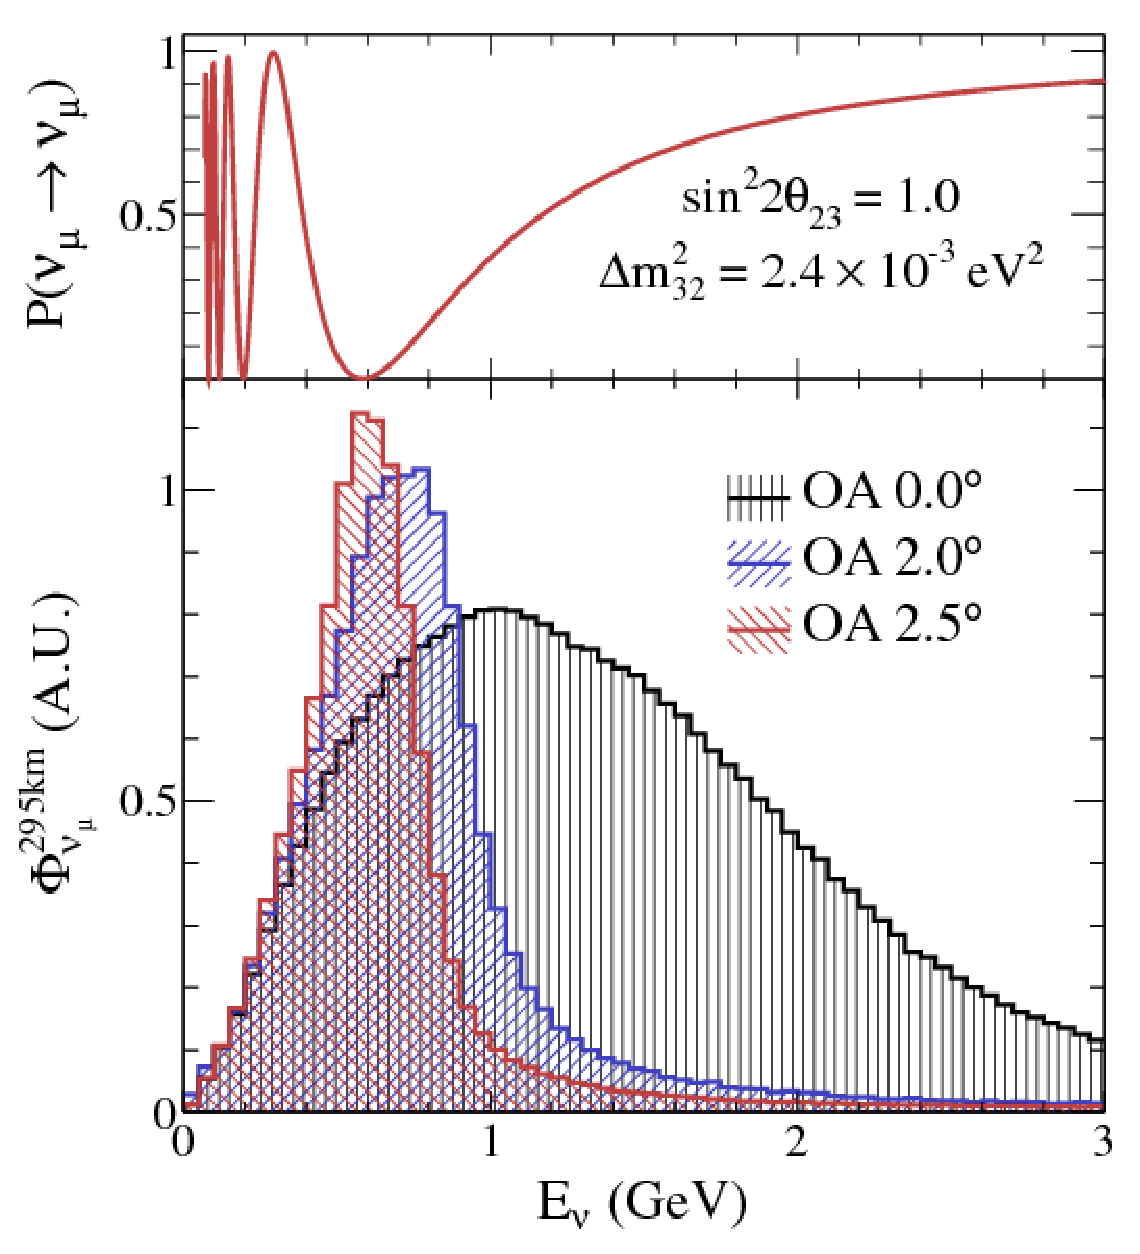
\includegraphics[width=0.8\columnwidth]{img/oaeffect_flux.eps}}
  }
  {
    % T2K detector
    \rput(0.425\slidewidth, 0.155\slideheight){\scalebox{0.75}{% T2K detector
\begin{pspicture}

  \psline[linewidth = 0.05, linecolor = pdcolor1](1.025,0)(1.025,2)
  \psline[linewidth = 0.05, linecolor = pdcolor1](2.975,0)(2.975,2)
  \psellipse[linewidth = 0.05, linecolor = pdcolor1](2,2)(1,0.2)
  \psellipse[linewidth = 0.05, linecolor = pdcolor1](2,0)(1,0.2)

  \psline[linewidth = 0.01, linecolor = pdcolor1]{|<->|}(1, -0.4)(3, -0.4)
  \rput[c](2,-0.6){\color{pdcolor1}\footnotesize $39.3$~m}
  \psline[linewidth = 0.01, linecolor = pdcolor1]{|<->|}(3.2,0)(3.2,2)
  \rput[l](3.4,1){\color{pdcolor1}\footnotesize $41.4$~m}

  \psline[linewidth = 0.03, linecolor = pdcolor4]{->}(0,1)(1.75,1)
  \rput[c](0.5,1.2){\color{pdcolor4}\footnotesize $\nu_\alpha$}

  \psline[linewidth = 0.03, linecolor = pdcolor4, linestyle = dotted]{-}(-3,1)(0,1)
  \rput[c](-1.5,1.2){\color{pdcolor4}\footnotesize 295 km}

  \psline[linewidth = 0.03, linecolor = pdcolor5]{->}(1.75,1)(2.5, 1.5)
  \rput[c]{45}(2,1.35){\color{pdcolor5}\footnotesize $\alpha$}
  \psline[linewidth = 0.03, linecolor = pdcolor3]{->}(1.75,1)(2.5, 0.75)
  \psline[linewidth = 0.03, linecolor = pdcolor3]{->}(1.75,1)(2.5, 0.5)
  \psline[linewidth = 0.03, linecolor = pdcolor3]{->}(1.75,1)(2.5, 0.25)

\end{pspicture}
}}

    \mbox{}\vspace{0.225\slideheight}  
  
    \begin{itemize}

      \item Off-axis beam
      \item Cherenkov detector (Super-Kamiokande)
      \item 50 000 tons of ultra-pure water
      \item Only charged leptons and final state charged hadrons are visible
      \item The neutrino energy is unknown
      
    \end{itemize}
  }
  
\end{wideslide}

%%%%% ENERGY RECONSTRUCTION %%%%%

\begin{slide}[toc=Energy reconstruction]{The problem with neutrino energy reconstruction}
 
  % SLIDE 1
  \onslide*{1}
  {
    \rput[c](13,3.5){% QEL vertex
\begin{pspicture}
  \rput[c](0,-1.75){Quasi-elastic scattering}
  \pscoil[coilarm = 0, linewidth = 0.025, linecolor = pdcolor1, coilwidth = 0.25, coilaspect = 0]{c-c}(-1,0)(1,0)
  \rput[c](0,-0.4){\color{pdcolor1}\small $W$}
  \psframe[linestyle = none, fillstyle = solid, fillcolor = pdcolor2](-1.1,-0.03)(-0.9,0.2)
  \psframe[linestyle = none, fillstyle = solid, fillcolor = pdcolor2](0.9,-0.03)(1.1,0.2)
  \pscircle[linestyle = none, fillstyle = solid, fillcolor = pdcolor1](-0.95,0){0.05}
  \pscircle[linestyle = none, fillstyle = solid, fillcolor = pdcolor1](0.95,0){0.05}
  \psline[linewidth = 0.025, linecolor = pdcolor1]{c-}(-0.95,0)(-2,1)
  \psline[linewidth = 0.025, linecolor = pdcolor1]{c-}(-0.95,0)(-2,-1)
  \psline[linewidth = 0.05, linecolor = pdcolor1]{c-}(0.95,0)(2,1)
  \psline[linewidth = 0.05, linecolor = pdcolor1]{c-}(0.95,0)(2,-1)
  
  \rput[l](-1.75,1){\color{pdcolor1} $l (k')$}
  \rput[l](-1.75,-1){\color{pdcolor1} $\nu (k)$}
  \rput[r](1.75,1){\color{pdcolor1} $p (p')$}
  \rput[r](1.75,-1){\color{pdcolor1} $n (p)$}

\end{pspicture}
}
    
    \mbox{} \\ \mbox{} \\
    
    In the case of neutrino scattering off \\ nucleon at rest neutrino energy can be \\ calculated from lepton kinematics:
    
    \mbox{} \\
    
    \twocolumn
    {
      \begin{eqnarray*}
	M_p^2 & = & p'^2 = (p + k - k')^2 \\ & & \\
	M_p^2 & = & m_l^2 + M_n^2 - 2M_nE_l \\
	& + & 2E_\nu(M_n - E_l + |\vec p_l|\cos\theta_l) \\ & & \\
	E_\nu & = & \frac{M_p^2 - M_n^2 - m_l^2 + 2M_nE_l}{2(M_n - E_l + |\vec p_l|\cos\theta_l)}
      \end{eqnarray*}
    }
    {
      \mbox{} \\ \mbox{} \\ \mbox{} \\
      \begin{eqnarray*}
	\hspace{20pt} k & = & (E_\nu, 0, 0, E_\nu) \\
	  k' & = & (E_l, \vec p_l) \\
	  p & = & (M_p, 0, 0, 0) \\
	  p' & = & p + q \\
	  q & = & k - k'       
      \end{eqnarray*}    
    }
  }
  % SLIDE 2-3 TOP
  \onslide*{2-3}
  {
    \rput(0.83\slidewidth, -0.075\slideheight){% nu-N scattering
\begin{pspicture}
      
  \rput[c](-1.5,0.3){\color{pdcolor4} $\nu$}
  \psline[linewidth = 0.03, linecolor = pdcolor4]{->}(-2,0)(0,0)
  
  \psline[linewidth = 0.03, linecolor = pdcolor1, linestyle = dotted](0,0)(3,0)
  \psarc[linewidth = 0.02, linecolor = pdcolor1, arrowscale = 0.75]{->}(0,0){2}{0}{18}
  \rput[l](2.2,0.35){\color{pdcolor1} $\theta_l$}

  
  \rput[c]{20}(1.7,0.85){\color{pdcolor5} $l$}
  \psline[linewidth = 0.03, linecolor = pdcolor5]{->}(0,0)(3,1)
  
  \rput[c]{-20}(1.8,-0.9){\color{pdcolor3} nucleon(s)}
  \psline[linewidth = 0.03, linecolor = pdcolor3]{->}(0,0)(3,-1)
  
  \rput[c]{-45}(0.13,-0.32){\color{pdcolor6} $\pi$}
  \psline[linewidth = 0.03, linecolor = pdcolor6]{->}(0,0)(0.5,-0.5)
  
  \rput[c](0,1.3){\color{pdcolor1} Nucleus}
  \onslide{2}{\pscircle[linewidth = 0.05, linecolor = pdcolor1, fillstyle = solid, fillcolor = pdcolor1](0,0){1}}
  \onslide{3}{\pscircle[linewidth = 0.05, linecolor = pdcolor1](0,0){1}}

\end{pspicture}
}
  
    \begin{itemize}
    
      \item Usually, the energy reconstruction procedure is based on quasi-elastic neutrino-nucleon scattering:
    
      $$E_\nu^{REC} = \frac{M_p^2 - (M_n - E_B)^2 - m_l^2 + 2(M_n - E_B)E_l}{2(M_n - E_B - E_l + |\vec p_l|\cos\theta_l)}$$

    \end{itemize}
  }
  % SLIDE 2
  \onslide*{2}
  {
    % COVER NUCLEUS
    \psframe[linewidth = 0.01, linecolor = pdcolor1](0,-2)(4,-1)
    \psframe[linewidth = 0.01, linecolor = pdcolor1](0,-3.1)(4,-2.1)
    \psframe[linewidth = 0.01, linecolor = pdcolor1](0,-3.2)(4,-4.2)
    % LABEL
    \rput[c](2,-1.5){\color{pdcolor1} Impulse Approximation}
    \rput[c](2,-2.6){\color{pdcolor1} No Fermi motion}
    \rput[c](2,-3.7){\color{pdcolor1} Binding Potential}
  }	
  
  \onslide*{3}
  {
    % LABEL
    \vspace{15pt}
    \psframe[linewidth = 0.01, linecolor = pdcolor1](-0.2,-2.8)(4.2,-1.2)
    \rput[c](2,-1.7){\color{pdcolor1} Never judge an event}
    \rput[c](2,-2.3){\color{pdcolor1} by its final state particles!}
  }
 
\end{slide}


%\section[toc=MC generators]{Monte Carlo generators}

%%%%% BUFFON'S NEEDLE PROBLEM %%%%

\begin{wideslide}{Buffon's needle problem}
\null\vfill

  \twocolumn
  {
    {\it Suppose we have a floor made of parallel strips of wood, each the same width, and we drop a needle onto the floor. What is the probability that the needle will lie across a line between two strips?}
    
    \sep
    
    {\it\hfill Georges-Louis Leclerc,\\\hfill Comte de Buffon\\\hfill 18th century}
  }
  {
    \sep\sep
    \centering\begin{tikzpicture}[node distance = 0cm]
 
  \node (a) [rectH, filled2=pdcolor1, line width = 0] {};
  \node (b) [rectH, notFilled=pdcolor1, line width = 0, right=of a] {};
  \node (c) [rectH, filled2=pdcolor1, line width = 0, right=of b] {};
  \node (d) [rectH, notFilled=pdcolor1, line width = 0, right=of c] {};
  \node (e) [rectH, filled2=pdcolor1, line width = 0, right=of d] {};
  \node (f) [rectH, notFilled=pdcolor1, line width = 0, right=of e] {};
  
  \draw[color = pdcolor7, ultra thick, xshift=0.1cm, yshift=0.0cm, rotate=45] (0,0) -- (0.4,0);
  \draw[color = pdcolor6, ultra thick, xshift=1.4cm, yshift=-0.8cm, rotate=35] (0,0) -- (0.4,0);
  \draw[color = pdcolor7, ultra thick, xshift=2.0cm, yshift=-0.4cm, rotate=-30] (0,0) -- (0.4,0);
  \draw[color = pdcolor6, ultra thick, xshift=2.5cm, yshift=0.6cm, rotate=60] (0,0) -- (0.4,0);
  \draw[color = pdcolor6, ultra thick, xshift=0.8cm, yshift=-0.5cm, rotate=-20] (0,0) -- (0.4,0);
  \draw[color = pdcolor7, ultra thick, xshift=1.1cm, yshift=0.3cm, rotate=15] (0,0) -- (0.4,0);
 
  \node(red) [below=of c, yshift=-0.1cm] {\color{pdcolor7} blue are good};
  \node(blue) [below=of red] {\color{pdcolor6} red are bad};
 
\end{tikzpicture}

  }
  
  \vspace{-10pt}
  \myBoxFullWidth{Monte Carlo without computers}
  
  \twocolumn
  {
    If needle length ($l$) $<$ lines width ($t$):
    
    $$P = \frac{2l}{t\pi}$$
    
    which can be used to estimate $\pi$:
    
    $$\pi = \frac{2l}{tP}$$
  }
  {
    MC experiment was performed by Mario Lazzarini in 1901 by throwing 3408 needles:
    
    $$\pi = \frac{2l \cdot 3408}{t \cdot \#red} = \frac{355}{113} = 3.14159292$$
  }
  
\vfill\null
\end{wideslide}

%%%%% STANISŁAM ULAM %%%%%

\begin{wideslide}[toc = From Solitaire to MC]{From Solitaire to Monte Carlo method}
\null\vfill

    \twocolumn
    {
      \begin{itemize}
	\item Stanis{\l}aw Ulam was a Polish mathematician
	\item He invented the Monte Carlo method while playing solitaire
	\item The method was used in Los Alamos, performed by ENIAC computer
      \end{itemize}  
      
      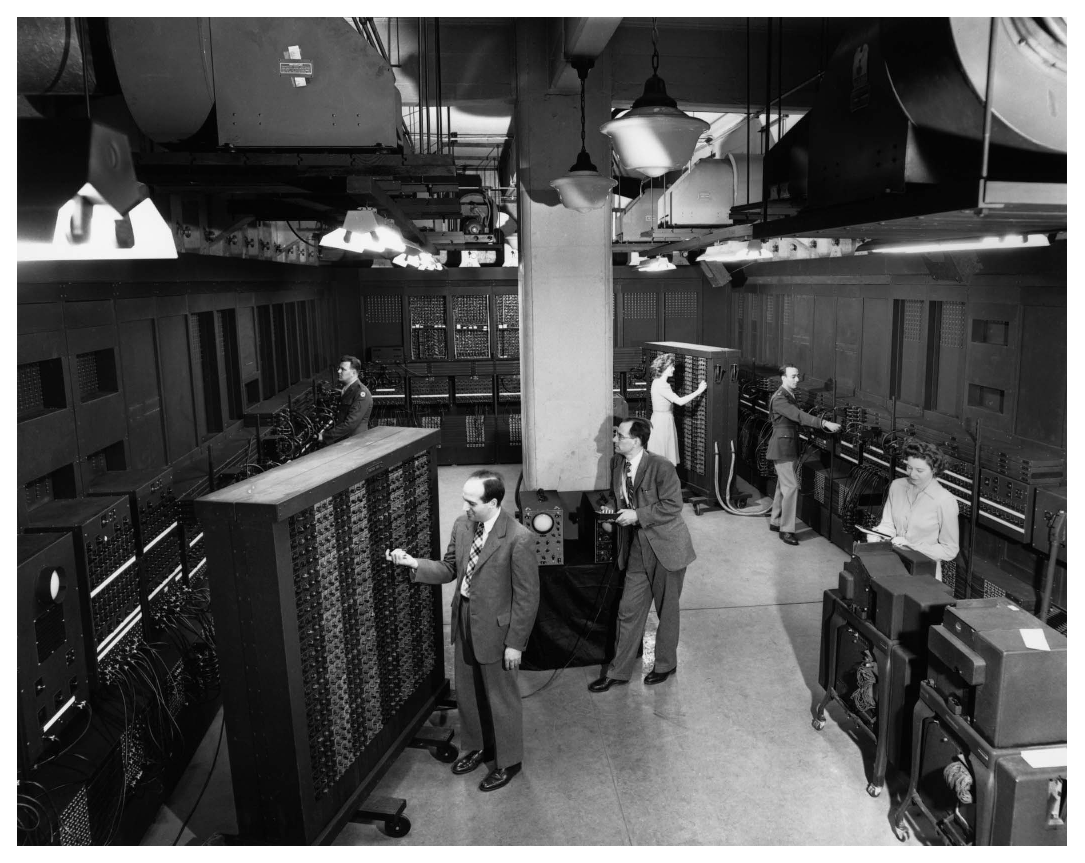
\includegraphics[width=\columnwidth]{img/eniac1946.eps}
    }
    {
      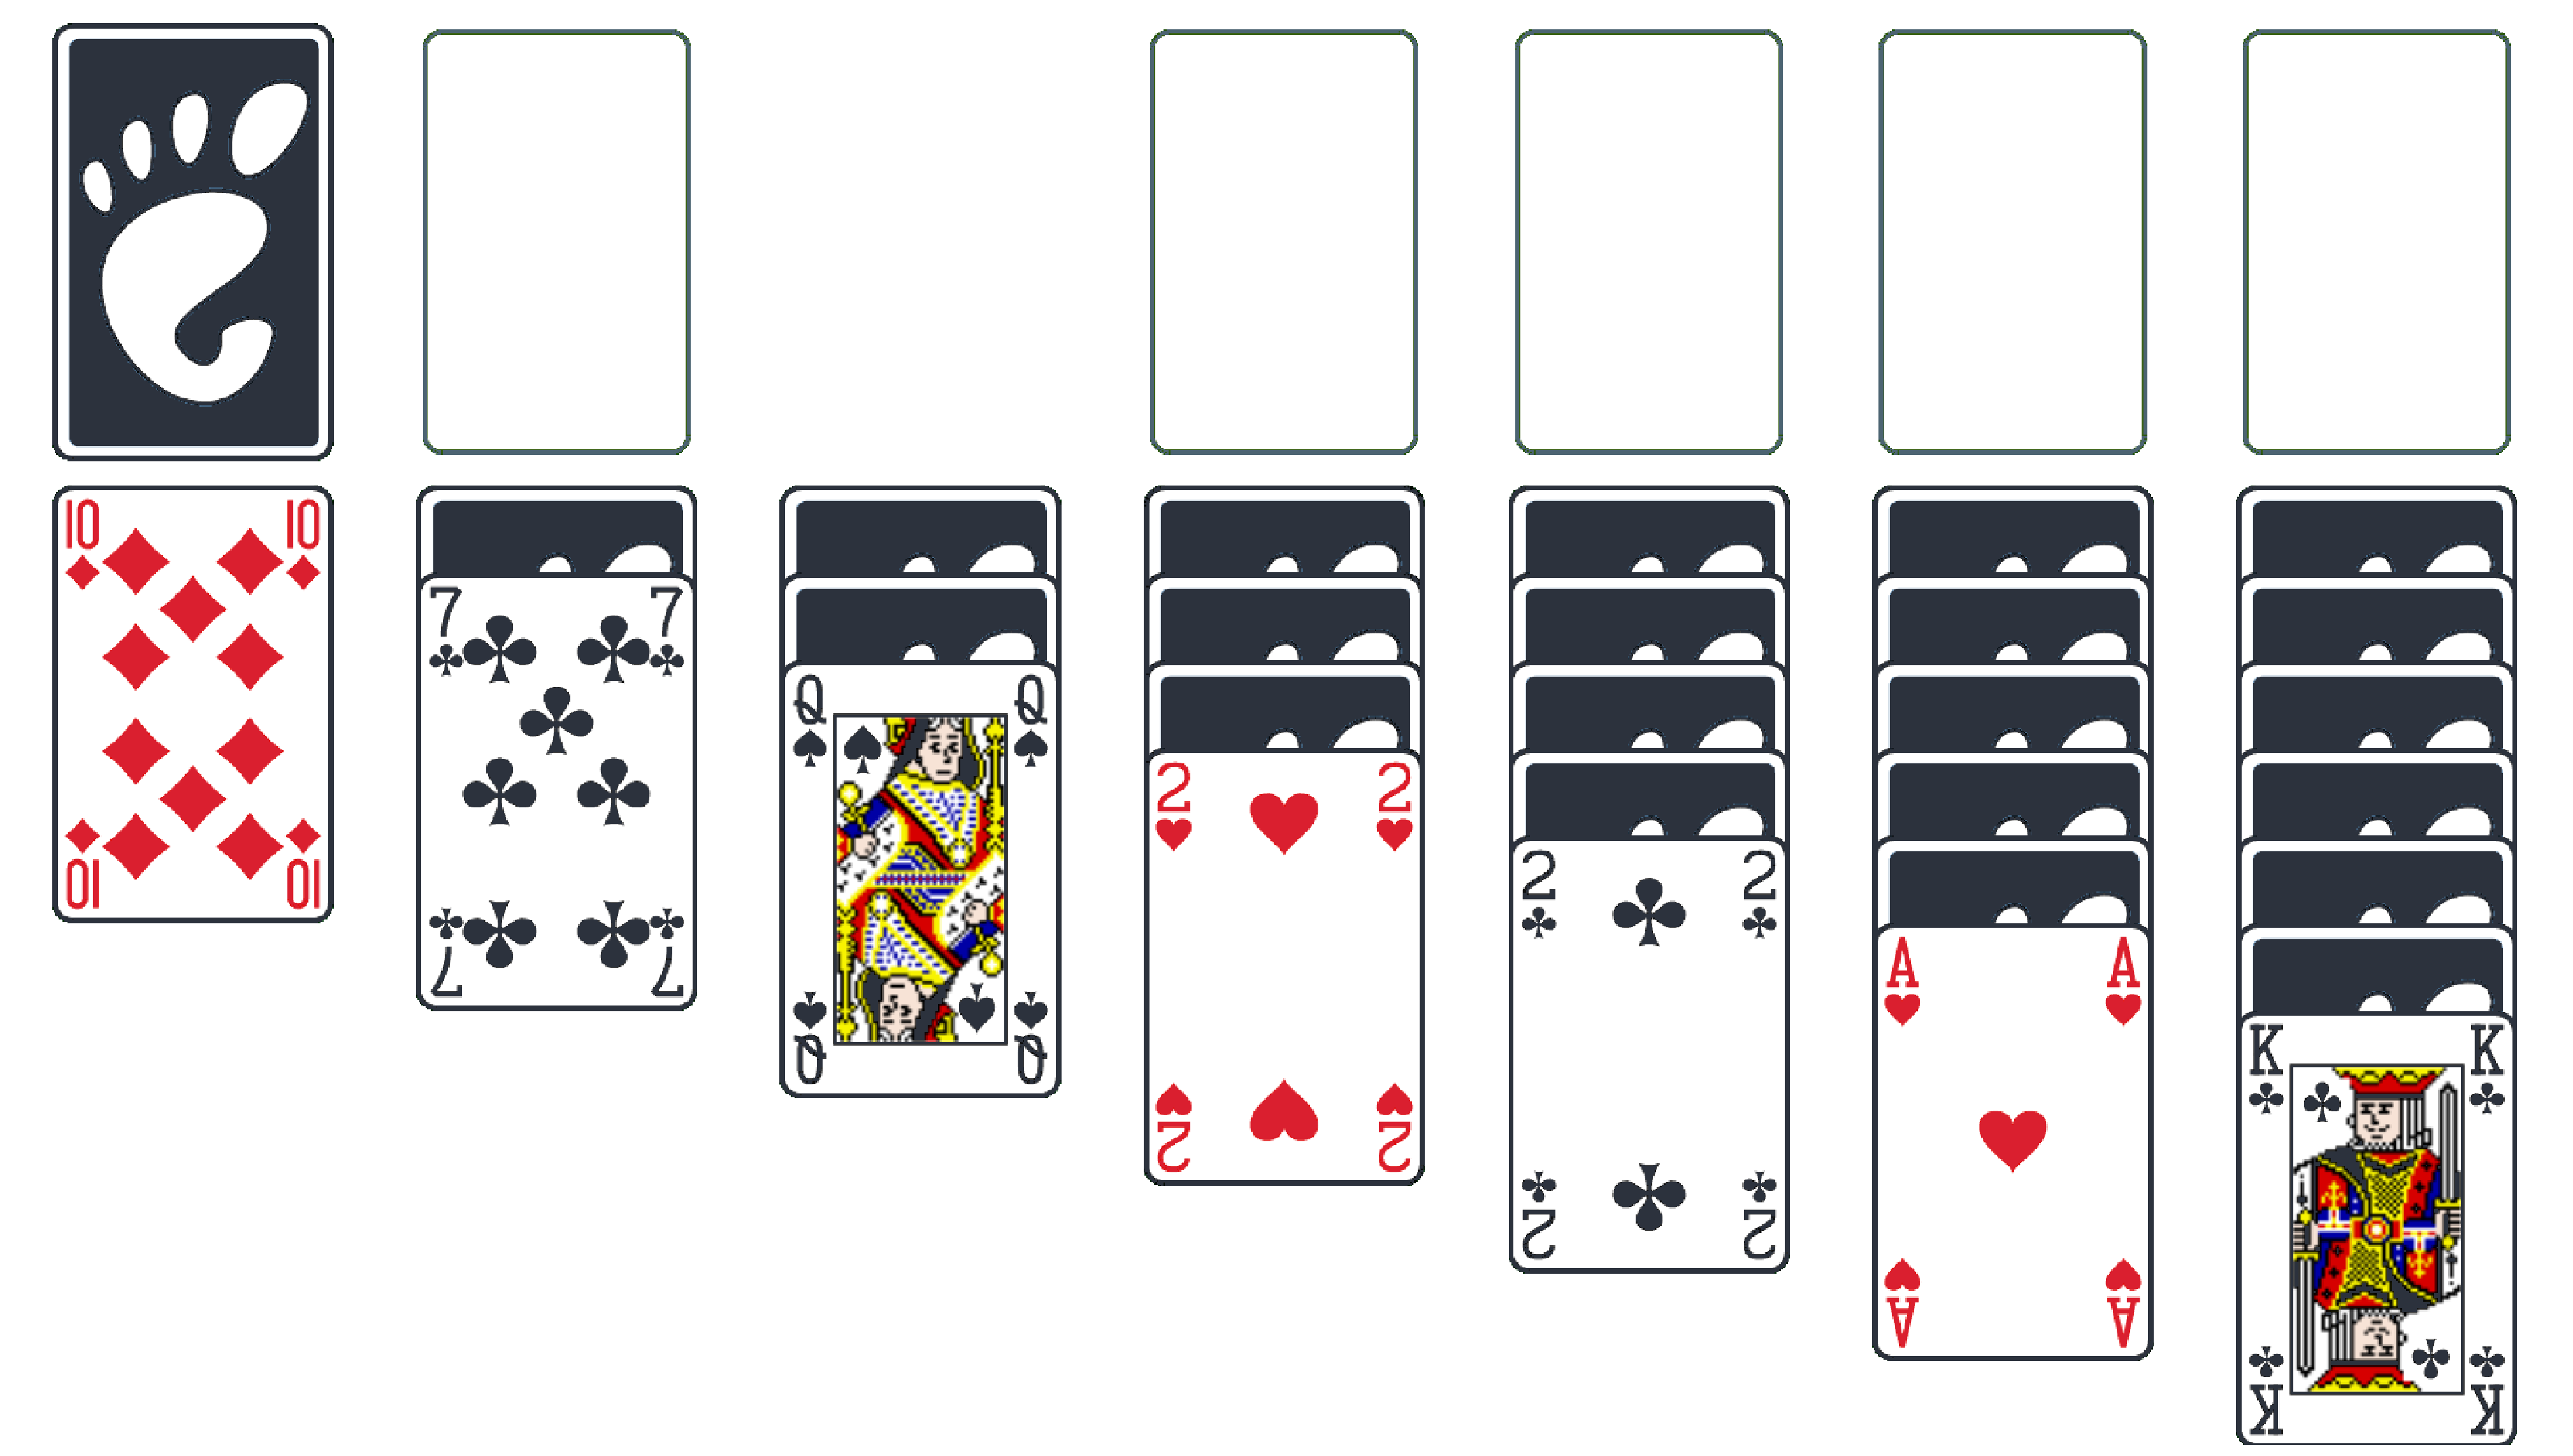
\includegraphics[width=\columnwidth]{img/solitaire.eps}
      \begin{itemize}
	\item What is a probability of success in solitaire?
	\begin{itemize}
	  \item Too complex for an analytical calculations
	  \item Lets try $N = 100$ times and count wins
	  \item With $N \rightarrow \infty$ we are getting closer to correct result
	\end{itemize}
      \end{itemize}
    }
 
\vfill\null
\end{wideslide}

%%%%% MC INTEGRATION: HIT-OR-MISS %%%%%

\begin{slide}[toc=Hit-or-miss method]{MC integration (hit-or-miss method)}
\null\vfill

  Lets do the following integration using MC method:
  
  $$\int_0^1 f(x)dx = \int_0^1 \left(\frac{1}{2}x\right) dx = \left.\frac{1}{2}\frac{x^2}{2}\right|_{0}^{1} = \frac{1}{4}$$

  \twocolumn
  {
    \sep
    \begin{itemize}
     \item take a random point from the $[0,1]\times[0,1]$ square
     \item compare it to your $f(x)$
     \item repeat $N$ times
     \item count $n$ points below the function
     \item you results is given by
     $$\int_0^1 f(x)dx = P_{\square} \cdot \frac{n}{N} = \frac{n}{N}$$
    \end{itemize}
  }
  {
    \usetikzlibrary{calc}

\begin{tikzpicture}

  \draw[>=latex, <->, thick] node[left, yshift = 4cm]{$y$} ++ (0, 4) -- (0, 0) -- node[below, xshift = 2cm]{$x$} ++ (4,0);
  
  \foreach \x in {1,...,200}
  {
    \pgfmathparse{rnd}
    \pgfmathsetmacro{\a}{2.9*\pgfmathresult + 0.05}
    \pgfmathparse{rnd}
    \pgfmathsetmacro{\b}{2.9*\pgfmathresult + 0.05}
    \pgfmathsetmacro{\c}{\a - 2.0 * \b}
        
    \ifthenelse{\lengthtest{\c pt > 0.2 pt}}{\draw[filled, color=pdcolor7] (\a, \b) circle (0.03);}{}
    \ifthenelse{\lengthtest{\c pt < - 0.2 pt}}{\draw[filled, color=pdcolor6] (\a, \b) circle (0.03);}{}
  }

  \draw[ultra thick] (0,0) -- node[yshift = 1.5cm, xshift = 2cm]{$f(x) = \frac{1}{2}x$} ++ (4,2);
  
  \draw[color=pdcolor3, dashed] node[left, yshift = 3cm]{1} ++ (0, 3) -- (3,3) -- node[yshift = -1.75cm]{1} (3, 0);
      
\end{tikzpicture}

  }
  
\vfill\null
\end{slide}

%%%%% MC INTEGRATION: CRUDE METHOD %%%%%

\begin{slide}[toc=Crude method]{MC integration (crude method)}
\null\vfill

  Lets do the following integration using MC method once again:
  
  $$\int_0^1 f(x)dx = \int_0^1 \left(\frac{1}{2}x\right) dx = \left.\frac{1}{2}\frac{x^2}{2}\right|_{0}^{1} = \frac{1}{4}$$
  \twocolumn
  {
    \begin{itemize}
      \item One can approximate integral
      \vspace{-5pt}
      $$\int_a^b f(x) dx \approx \frac{b - a}{N}\sum_{i=1}^{N} f(x_i)$$
     
      where $x_i$ is a random number from $[a, b]$
      
      \item It can be shown that crude method is more accurate than hit-or-miss
      
      \item We will skip the math and look at some comparisons
      
    \end{itemize}
  }
  {
    \usetikzlibrary{calc}

\begin{tikzpicture}

  \draw[>=latex, <->, thick] node[left, yshift = 4cm]{$y$} ++ (0, 4) -- (0, 0) -- node[below, xshift = 2cm]{$x$} ++ (4,0);
  
  \foreach \x in {1,...,14}
  {
    \pgfmathparse{rnd}

    \pgfmathsetmacro{\a}{0.2 * \x + 0.05 + 0.1 * \pgfmathresult - 0.05}
        
    \draw[filled, color=pdcolor7] (\a, 0) circle (0.03);
    
    \draw[thin, color=pdcolor3, dashed] (\a, 0) -- (\a, 0.5*\a);
  }

  \draw[ultra thick] (0,0) -- node[yshift = 1.5cm, xshift = 2cm]{$f(x) = \frac{1}{2}x$} ++ (4,2);
        
\end{tikzpicture}

  }

\vfill\null
\end{slide}

%%%%% HIT-OR-MISS vs CRUDE %%%%%

\begin{emptyslide}{Methods comparison}
\null\vfill

  \twocolumn
  {
    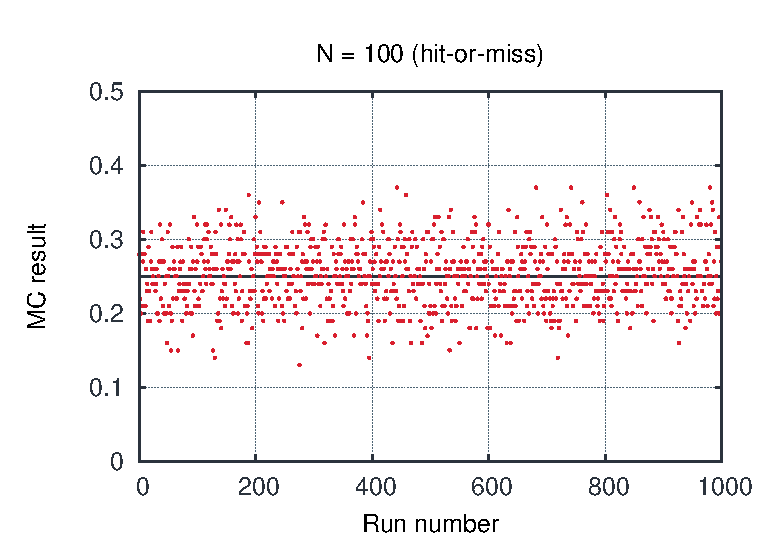
\includegraphics[width=\columnwidth]{img/int100.eps}
    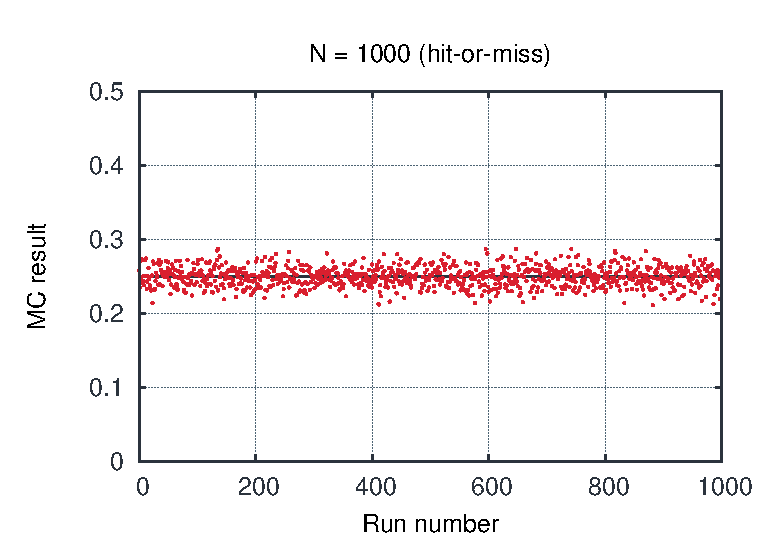
\includegraphics[width=\columnwidth]{img/int1000.eps}
  }
  {
    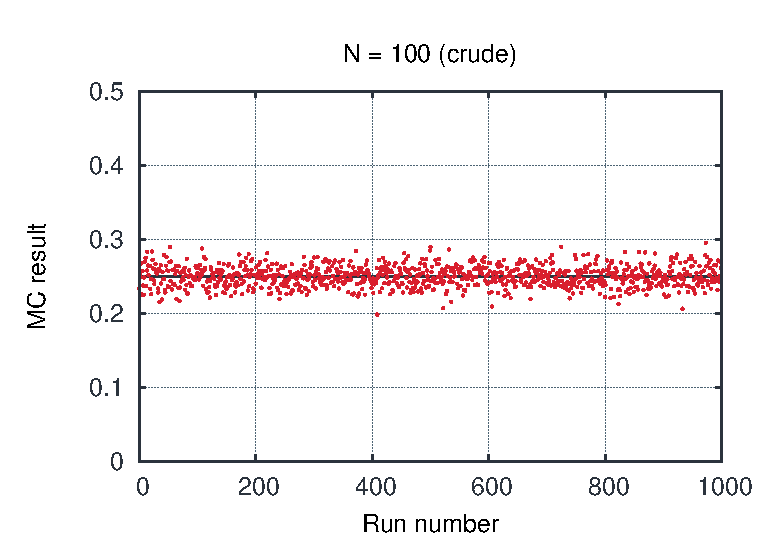
\includegraphics[width=\columnwidth]{img/int2100.eps}
    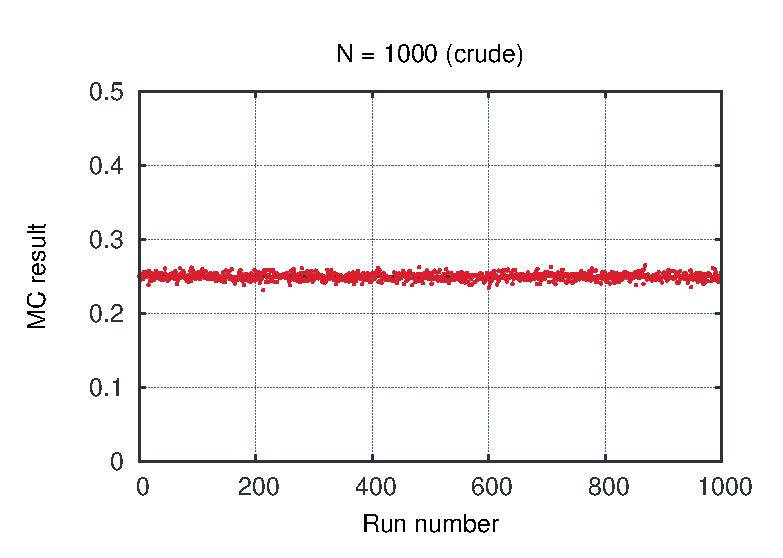
\includegraphics[width=\columnwidth]{img/int21000.eps}
  }

\vfill\null
\end{emptyslide}

%%%%% ACCEPT-REJECT %%%%%

\begin{slide}[toc=]{Acceptance-rejection method}
\null\vfill

  \twocolumn
  {
    \myFrameFullWidth{For generating events \\ according to a distribution.}
    
    \begin{itemize}
      \item Evaluate $f_{max} \geq \mbox{max}(f)$
      \item[] {\it\color{pdcolor3}Note: $f_{max} > \mbox{max}(f)$ will affect performance, but the result will be still correct}
      \item Generate random $x$
      \item Accept $x$ with $P = \frac{f(x)}{f_{max}}$
      \begin{itemize}
	\item generate a random $u$ from $[0, f_{max}]$
	\item accept if $u < f(x)$
      \end{itemize}
    \end{itemize}
  }
  {
    \usetikzlibrary{calc}

\pgfplotsset{every  tick/.style={pdcolor3,}, minor x tick num=1,}

\begin{tikzpicture}

  \begin{axis}[xlabel = {$x$}, ylabel = {$y$}, ylabel near ticks, domain=0:1, scale=0.5, axis lines = left, inner axis line style={>=latex}, ymin = 0, ymax = 0.75, xmin = 0, xmax = 1.1]

    \addplot[mark=none, dashed, color=pdcolor3, thick] coordinates {(0,0.6) (1,0.6) (1,0)};

    \node[above] at (axis cs: 0.5, 0.6) {$f_{max}$};

    \addplot [thick, mark = none, color = pdcolor1] {x*x*x*exp(-x*x)};
    \node[above] at (axis cs: 0.5, 0.3) {\small$f(x) = x^3\cdot e^{-x^2}$};
    
  \end{axis}

\end{tikzpicture}
    \usetikzlibrary{calc}

\pgfplotsset{every  tick/.style={pdcolor3,}, minor x tick num=1,}

\begin{tikzpicture}

  \begin{axis}[xlabel = {$x$}, ylabel = {$y$}, ylabel near ticks, domain=0:1, scale=0.5, axis lines = left, inner axis line style={>=latex}, ymin = 0, ymax = 0.45, xmin = 0, xmax = 1.1]
    
    \addplot [thick, color = pdcolor6] table[x = x, y = y, col sep = space, mark = none] {data/ar.dat};
    \addplot [dashed, mark = none, color = pdcolor1] {x*x*x*exp(-x*x)};
    
  \end{axis}

\end{tikzpicture}
  }

\vfill\null
\end{slide}

%%%%% MC GENERATORS %%%%%

\begin{slide}[toc=MC generators]{Monte Carlo event generators}
\null\vfill

  \rput(1.1\slidewidth, 0.6\slideheight){\scalebox{1.5}{\begin{pspicture}
  \pscircle[linewidth = 0.05, linecolor = pdcolor1](0,0){1}

  \psline[linewidth = 0.05, linecolor = pdcolor4]{->}(-1.6,0)(-1.1,0)
  \psline[linewidth = 0.05, linecolor = pdcolor5]{->}(1.1,0.5)(1.6,0.75)
  \psline[linewidth = 0.05, linecolor = pdcolor5]{->}(1.1,0)(1.6,0)
  \psline[linewidth = 0.05, linecolor = pdcolor5]{->}(1.1,-0.5)(1.6,-0.75)
  
  \rput[c](0,0){\scalebox{0.075}{%LaTeX with PSTricks extensions
%%Creator: inkscape 0.48.4
%%Please note this file requires PSTricks extensions
\psset{xunit=.5pt,yunit=.5pt,runit=.5pt}
\begin{pspicture}(1024,1024)
{
\newrgbcolor{curcolor}{0.12941177 0.14509805 0.19607843}
\pscustom[linestyle=none,fillstyle=solid,fillcolor=curcolor]
{
\newpath
\moveto(476.52942,979.76519)
\curveto(487.77942,998.51519)(514.02942,1021.01519)(532.77942,1021.01519)
\lineto(945.27942,788.51519)
\curveto(952.77942,781.01519)(971.52942,732.26519)(956.52942,713.51519)
\lineto(547.77942,473.51519)
\curveto(536.52942,469.76519)(487.77942,473.51519)(472.77942,511.01519)
\lineto(476.52942,979.76519)
\closepath
}
}
{
\newrgbcolor{curcolor}{0.12941177 0.14509805 0.19607843}
\pscustom[linewidth=3,linecolor=curcolor]
{
\newpath
\moveto(476.52942,979.76519)
\curveto(487.77942,998.51519)(514.02942,1021.01519)(532.77942,1021.01519)
\lineto(945.27942,788.51519)
\curveto(952.77942,781.01519)(971.52942,732.26519)(956.52942,713.51519)
\lineto(547.77942,473.51519)
\curveto(536.52942,469.76519)(487.77942,473.51519)(472.77942,511.01519)
\lineto(476.52942,979.76519)
\closepath
}
}
{
\newrgbcolor{curcolor}{1 1 1}
\pscustom[linestyle=none,fillstyle=solid,fillcolor=curcolor]
{
\newpath
\moveto(517.1383,502.04801)
\curveto(506.42376,483.44891)(488.892,483.44915)(478.17747,502.04825)
\lineto(359.4827,708.08751)
\curveto(348.76859,726.68588)(348.76816,757.11932)(359.4827,775.7184)
\lineto(478.17747,981.75767)
\curveto(488.89172,1000.356275)(506.42418,1000.356275)(517.1383,981.75791)
\lineto(635.83307,775.71865)
\curveto(646.54761,757.11956)(646.54732,726.68588)(635.83307,708.08728)
\lineto(517.1383,502.04801)
\closepath
}
}
{
\newrgbcolor{curcolor}{0.12941177 0.14509805 0.19607843}
\pscustom[linewidth=3.73868561,linecolor=curcolor]
{
\newpath
\moveto(517.1383,502.04801)
\curveto(506.42376,483.44891)(488.892,483.44915)(478.17747,502.04825)
\lineto(359.4827,708.08751)
\curveto(348.76859,726.68588)(348.76816,757.11932)(359.4827,775.7184)
\lineto(478.17747,981.75767)
\curveto(488.89172,1000.356275)(506.42418,1000.356275)(517.1383,981.75791)
\lineto(635.83307,775.71865)
\curveto(646.54761,757.11956)(646.54732,726.68588)(635.83307,708.08728)
\lineto(517.1383,502.04801)
\closepath
}
}
{
\newrgbcolor{curcolor}{0.12941177 0.14509805 0.19607843}
\pscustom[linestyle=none,fillstyle=solid,fillcolor=curcolor]
{
\newpath
\moveto(514.02984324,770.32250396)
\curveto(523.07178558,754.62682324)(523.07178558,729.17909676)(514.02984324,713.48341604)
\curveto(504.98790089,697.78773531)(490.32801581,697.78773531)(481.28607346,713.48341604)
\curveto(472.24413112,729.17909676)(472.24413112,754.62682324)(481.28607346,770.32250396)
\curveto(490.32801581,786.01818469)(504.98790089,786.01818469)(514.02984324,770.32250396)
\closepath
}
}
{
\newrgbcolor{curcolor}{0.12941177 0.14509805 0.19607843}
\pscustom[linewidth=2.67048985,linecolor=curcolor]
{
\newpath
\moveto(514.02984324,770.32250396)
\curveto(523.07178558,754.62682324)(523.07178558,729.17909676)(514.02984324,713.48341604)
\curveto(504.98790089,697.78773531)(490.32801581,697.78773531)(481.28607346,713.48341604)
\curveto(472.24413112,729.17909676)(472.24413112,754.62682324)(481.28607346,770.32250396)
\curveto(490.32801581,786.01818469)(504.98790089,786.01818469)(514.02984324,770.32250396)
\closepath
}
}
{
\newrgbcolor{curcolor}{1 1 1}
\pscustom[linestyle=none,fillstyle=solid,fillcolor=curcolor]
{
\newpath
\moveto(936.13332,746.70165)
\curveto(957.59787,746.72225)(966.36354,731.53907)(955.61352,712.96046)
\lineto(836.52566,507.14816)
\curveto(825.77606,488.57028)(799.42013,473.35319)(777.95558,473.33272)
\lineto(540.17294,473.10577)
\curveto(518.70894,473.08527)(509.9427,488.26883)(520.6923,506.8467)
\lineto(639.78018,712.65902)
\curveto(650.5302,731.23763)(676.88668,746.45421)(698.35068,746.4747)
\lineto(936.13332,746.70165)
\closepath
}
}
{
\newrgbcolor{curcolor}{0.12941177 0.14509805 0.19607843}
\pscustom[linewidth=3.73868561,linecolor=curcolor]
{
\newpath
\moveto(936.13332,746.70165)
\curveto(957.59787,746.72225)(966.36354,731.53907)(955.61352,712.96046)
\lineto(836.52566,507.14816)
\curveto(825.77606,488.57028)(799.42013,473.35319)(777.95558,473.33272)
\lineto(540.17294,473.10577)
\curveto(518.70894,473.08527)(509.9427,488.26883)(520.6923,506.8467)
\lineto(639.78018,712.65902)
\curveto(650.5302,731.23763)(676.88668,746.45421)(698.35068,746.4747)
\lineto(936.13332,746.70165)
\closepath
}
}
{
\newrgbcolor{curcolor}{0.12941177 0.14509805 0.19607843}
\pscustom[linestyle=none,fillstyle=solid,fillcolor=curcolor]
{
\newpath
\moveto(844.51944383,690.21935432)
\curveto(853.59133236,705.89774585)(875.62971231,718.62160859)(893.74354319,718.63889718)
\curveto(911.85737406,718.65618578)(919.1873166,705.96035337)(910.11542807,690.28196184)
\curveto(901.04353955,674.60357031)(879.00515959,661.87970757)(860.89132872,661.86241898)
\curveto(842.77749785,661.84513038)(835.44755531,674.54096278)(844.51944383,690.21935432)
\closepath
}
}
{
\newrgbcolor{curcolor}{0.12941177 0.14509805 0.19607843}
\pscustom[linewidth=2.67048991,linecolor=curcolor]
{
\newpath
\moveto(844.51944383,690.21935432)
\curveto(853.59133236,705.89774585)(875.62971231,718.62160859)(893.74354319,718.63889718)
\curveto(911.85737406,718.65618578)(919.1873166,705.96035337)(910.11542807,690.28196184)
\curveto(901.04353955,674.60357031)(879.00515959,661.87970757)(860.89132872,661.86241898)
\curveto(842.77749785,661.84513038)(835.44755531,674.54096278)(844.51944383,690.21935432)
\closepath
}
}
{
\newrgbcolor{curcolor}{0.12941177 0.14509805 0.19607843}
\pscustom[linestyle=none,fillstyle=solid,fillcolor=curcolor]
{
\newpath
\moveto(659.06885402,690.04235259)
\curveto(668.14074254,705.72074412)(690.1791225,718.44460686)(708.29295337,718.46189545)
\curveto(726.40678424,718.47918404)(733.73672678,705.78335164)(724.66483825,690.10496011)
\curveto(715.59294973,674.42656858)(693.55456977,661.70270584)(675.4407389,661.68541724)
\curveto(657.32690803,661.66812865)(649.99696549,674.36396105)(659.06885402,690.04235259)
\closepath
}
}
{
\newrgbcolor{curcolor}{0.12941177 0.14509805 0.19607843}
\pscustom[linewidth=2.67048991,linecolor=curcolor]
{
\newpath
\moveto(659.06885402,690.04235259)
\curveto(668.14074254,705.72074412)(690.1791225,718.44460686)(708.29295337,718.46189545)
\curveto(726.40678424,718.47918404)(733.73672678,705.78335164)(724.66483825,690.10496011)
\curveto(715.59294973,674.42656858)(693.55456977,661.70270584)(675.4407389,661.68541724)
\curveto(657.32690803,661.66812865)(649.99696549,674.36396105)(659.06885402,690.04235259)
\closepath
}
}
{
\newrgbcolor{curcolor}{0.12941177 0.14509805 0.19607843}
\pscustom[linestyle=none,fillstyle=solid,fillcolor=curcolor]
{
\newpath
\moveto(566.19124479,529.52570903)
\curveto(575.26305576,545.20396653)(597.30124731,557.92772049)(615.41492332,557.94500894)
\curveto(633.52859934,557.96229738)(640.85847921,545.26657352)(631.78666825,529.58831602)
\curveto(622.71485728,513.91005852)(600.67666573,501.18630456)(582.56298971,501.16901611)
\curveto(564.44931369,501.15172767)(557.11943382,513.84745153)(566.19124479,529.52570903)
\closepath
}
}
{
\newrgbcolor{curcolor}{0.12941177 0.14509805 0.19607843}
\pscustom[linewidth=2.67048991,linecolor=curcolor]
{
\newpath
\moveto(566.19124479,529.52570903)
\curveto(575.26305576,545.20396653)(597.30124731,557.92772049)(615.41492332,557.94500894)
\curveto(633.52859934,557.96229738)(640.85847921,545.26657352)(631.78666825,529.58831602)
\curveto(622.71485728,513.91005852)(600.67666573,501.18630456)(582.56298971,501.16901611)
\curveto(564.44931369,501.15172767)(557.11943382,513.84745153)(566.19124479,529.52570903)
\closepath
}
}
{
\newrgbcolor{curcolor}{0.12941177 0.14509805 0.19607843}
\pscustom[linestyle=none,fillstyle=solid,fillcolor=curcolor]
{
\newpath
\moveto(705.35499371,609.87241006)
\curveto(714.42688223,625.55080159)(736.46526219,638.27466434)(754.57909306,638.29195293)
\curveto(772.69292393,638.30924152)(780.02286647,625.61340912)(770.95097794,609.93501759)
\curveto(761.87908942,594.25662605)(739.84070946,581.53276331)(721.72687859,581.51547472)
\curveto(703.61304772,581.49818613)(696.28310518,594.19401853)(705.35499371,609.87241006)
\closepath
}
}
{
\newrgbcolor{curcolor}{0.12941177 0.14509805 0.19607843}
\pscustom[linewidth=2.67048991,linecolor=curcolor]
{
\newpath
\moveto(705.35499371,609.87241006)
\curveto(714.42688223,625.55080159)(736.46526219,638.27466434)(754.57909306,638.29195293)
\curveto(772.69292393,638.30924152)(780.02286647,625.61340912)(770.95097794,609.93501759)
\curveto(761.87908942,594.25662605)(739.84070946,581.53276331)(721.72687859,581.51547472)
\curveto(703.61304772,581.49818613)(696.28310518,594.19401853)(705.35499371,609.87241006)
\closepath
}
}
{
\newrgbcolor{curcolor}{0.12941177 0.14509805 0.19607843}
\pscustom[linestyle=none,fillstyle=solid,fillcolor=curcolor]
{
\newpath
\moveto(751.64078083,529.70258469)
\curveto(760.71270813,545.38104323)(782.75118229,558.10496037)(800.86509059,558.12224903)
\curveto(818.97899889,558.1395377)(826.30897276,545.44365103)(817.23704546,529.76519248)
\curveto(808.16511816,514.08673393)(786.126644,501.3628168)(768.0127357,501.34552813)
\curveto(749.89882739,501.32823947)(742.56885352,514.02412614)(751.64078083,529.70258469)
\closepath
}
}
{
\newrgbcolor{curcolor}{0.12941177 0.14509805 0.19607843}
\pscustom[linewidth=2.67048991,linecolor=curcolor]
{
\newpath
\moveto(751.64078083,529.70258469)
\curveto(760.71270813,545.38104323)(782.75118229,558.10496037)(800.86509059,558.12224903)
\curveto(818.97899889,558.1395377)(826.30897276,545.44365103)(817.23704546,529.76519248)
\curveto(808.16511816,514.08673393)(786.126644,501.3628168)(768.0127357,501.34552813)
\curveto(749.89882739,501.32823947)(742.56885352,514.02412614)(751.64078083,529.70258469)
\closepath
}
}
{
\newrgbcolor{curcolor}{1 1 1}
\pscustom[linestyle=none,fillstyle=solid,fillcolor=curcolor]
{
\newpath
\moveto(514.94154,986.827505)
\curveto(504.19152,1005.4061)(512.95761,1020.588935)(534.42218,1020.568445)
\lineto(772.20482,1020.341495)
\curveto(793.66853,1020.321095)(820.02488,1005.10466)(830.7749,986.52605)
\lineto(949.86276,780.71375)
\curveto(960.61251,762.13564)(951.84627,746.95207)(930.38256,746.97256)
\lineto(692.59992,747.19951)
\curveto(671.13535,747.22)(644.77916,762.43708)(634.02942,781.01519)
\lineto(514.94154,986.827505)
\closepath
}
}
{
\newrgbcolor{curcolor}{0.12941177 0.14509805 0.19607843}
\pscustom[linewidth=3.73868561,linecolor=curcolor]
{
\newpath
\moveto(514.94154,986.827505)
\curveto(504.19152,1005.4061)(512.95761,1020.588935)(534.42218,1020.568445)
\lineto(772.20482,1020.341495)
\curveto(793.66853,1020.321095)(820.02488,1005.10466)(830.7749,986.52605)
\lineto(949.86276,780.71375)
\curveto(960.61251,762.13564)(951.84627,746.95207)(930.38256,746.97256)
\lineto(692.59992,747.19951)
\curveto(671.13535,747.22)(644.77916,762.43708)(634.02942,781.01519)
\lineto(514.94154,986.827505)
\closepath
}
}
{
\newrgbcolor{curcolor}{0.12941177 0.14509805 0.19607843}
\pscustom[linestyle=none,fillstyle=solid,fillcolor=curcolor]
{
\newpath
\moveto(609.663603,935.72872148)
\curveto(591.54977213,935.74601007)(569.51139217,948.46987282)(560.43950365,964.14826435)
\curveto(551.36761513,979.82665588)(558.69755766,992.52248828)(576.81138854,992.50519969)
\curveto(594.92521941,992.4879111)(616.96359937,979.76404835)(626.03548789,964.08565682)
\curveto(635.10737641,948.40726529)(627.77743388,935.71143289)(609.663603,935.72872148)
\closepath
}
}
{
\newrgbcolor{curcolor}{0.12941177 0.14509805 0.19607843}
\pscustom[linewidth=2.67048991,linecolor=curcolor]
{
\newpath
\moveto(609.663603,935.72872148)
\curveto(591.54977213,935.74601007)(569.51139217,948.46987282)(560.43950365,964.14826435)
\curveto(551.36761513,979.82665588)(558.69755766,992.52248828)(576.81138854,992.50519969)
\curveto(594.92521941,992.4879111)(616.96359937,979.76404835)(626.03548789,964.08565682)
\curveto(635.10737641,948.40726529)(627.77743388,935.71143289)(609.663603,935.72872148)
\closepath
}
}
{
\newrgbcolor{curcolor}{0.12941177 0.14509805 0.19607843}
\pscustom[linestyle=none,fillstyle=solid,fillcolor=curcolor]
{
\newpath
\moveto(702.54219337,775.21231955)
\curveto(684.4283625,775.22960814)(662.38998254,787.95347088)(653.31809402,803.63186241)
\curveto(644.24620549,819.31025395)(651.57614803,832.00608635)(669.6899789,831.98879776)
\curveto(687.80380977,831.97150916)(709.84218973,819.24764642)(718.91407825,803.56925489)
\curveto(727.98596678,787.89086336)(720.65602424,775.19503096)(702.54219337,775.21231955)
\closepath
}
}
{
\newrgbcolor{curcolor}{0.12941177 0.14509805 0.19607843}
\pscustom[linewidth=2.67048991,linecolor=curcolor]
{
\newpath
\moveto(702.54219337,775.21231955)
\curveto(684.4283625,775.22960814)(662.38998254,787.95347088)(653.31809402,803.63186241)
\curveto(644.24620549,819.31025395)(651.57614803,832.00608635)(669.6899789,831.98879776)
\curveto(687.80380977,831.97150916)(709.84218973,819.24764642)(718.91407825,803.56925489)
\curveto(727.98596678,787.89086336)(720.65602424,775.19503096)(702.54219337,775.21231955)
\closepath
}
}
{
\newrgbcolor{curcolor}{0.12941177 0.14509805 0.19607843}
\pscustom[linestyle=none,fillstyle=solid,fillcolor=curcolor]
{
\newpath
\moveto(887.99250187,775.03628832)
\curveto(869.87882585,775.05357676)(847.8406343,787.77733073)(838.76882333,803.45558823)
\curveto(829.69701236,819.13384572)(837.02689224,831.82956959)(855.14056825,831.81228114)
\curveto(873.25424427,831.7949927)(895.29243582,819.07123873)(904.36424679,803.39298123)
\curveto(913.43605776,787.71472374)(906.10617788,775.01899988)(887.99250187,775.03628832)
\closepath
}
}
{
\newrgbcolor{curcolor}{0.12941177 0.14509805 0.19607843}
\pscustom[linewidth=2.67048991,linecolor=curcolor]
{
\newpath
\moveto(887.99250187,775.03628832)
\curveto(869.87882585,775.05357676)(847.8406343,787.77733073)(838.76882333,803.45558823)
\curveto(829.69701236,819.13384572)(837.02689224,831.82956959)(855.14056825,831.81228114)
\curveto(873.25424427,831.7949927)(895.29243582,819.07123873)(904.36424679,803.39298123)
\curveto(913.43605776,787.71472374)(906.10617788,775.01899988)(887.99250187,775.03628832)
\closepath
}
}
{
\newrgbcolor{curcolor}{0.12941177 0.14509805 0.19607843}
\pscustom[linestyle=none,fillstyle=solid,fillcolor=curcolor]
{
\newpath
\moveto(795.11454758,935.55184069)
\curveto(777.00063927,935.56912936)(754.96216511,948.29304649)(745.89023781,963.97150504)
\curveto(736.81831051,979.64996359)(744.14828438,992.34585026)(762.26219268,992.32856159)
\curveto(780.37610098,992.31127293)(802.41457514,979.58735579)(811.48650244,963.90889724)
\curveto(820.55842975,948.23043869)(813.22845588,935.53455203)(795.11454758,935.55184069)
\closepath
}
}
{
\newrgbcolor{curcolor}{0.12941177 0.14509805 0.19607843}
\pscustom[linewidth=2.67048991,linecolor=curcolor]
{
\newpath
\moveto(795.11454758,935.55184069)
\curveto(777.00063927,935.56912936)(754.96216511,948.29304649)(745.89023781,963.97150504)
\curveto(736.81831051,979.64996359)(744.14828438,992.34585026)(762.26219268,992.32856159)
\curveto(780.37610098,992.31127293)(802.41457514,979.58735579)(811.48650244,963.90889724)
\curveto(820.55842975,948.23043869)(813.22845588,935.53455203)(795.11454758,935.55184069)
\closepath
}
}
{
\newrgbcolor{curcolor}{0.12941177 0.14509805 0.19607843}
\pscustom[linestyle=none,fillstyle=solid,fillcolor=curcolor]
{
\newpath
\moveto(654.69727,487.8886)
\curveto(673.44727,476.6386)(695.94727,450.3886)(695.94727,431.6386)
\lineto(454.70688,13.6148)
\curveto(444.71994,7.4401)(423.08878,-4.9951)(392.3516,5.6702)
\lineto(148.44727,416.6386)
\curveto(144.69727,427.8886)(148.44727,476.6386)(185.94727,491.6386)
\lineto(654.69727,487.8886)
\closepath
}
}
{
\newrgbcolor{curcolor}{0.12941177 0.14509805 0.19607843}
\pscustom[linewidth=3,linecolor=curcolor]
{
\newpath
\moveto(654.69727,487.8886)
\curveto(673.44727,476.6386)(695.94727,450.3886)(695.94727,431.6386)
\lineto(454.70688,13.6148)
\curveto(444.71994,7.4401)(423.08878,-4.9951)(392.3516,5.6702)
\lineto(148.44727,416.6386)
\curveto(144.69727,427.8886)(148.44727,476.6386)(185.94727,491.6386)
\lineto(654.69727,487.8886)
\closepath
}
}
{
\newrgbcolor{curcolor}{1 1 1}
\pscustom[linestyle=none,fillstyle=solid,fillcolor=curcolor]
{
\newpath
\moveto(176.98009,447.27972)
\curveto(158.38099,457.99426)(158.38123,475.52602)(176.98033,486.24056)
\lineto(383.01959,604.93533)
\curveto(401.61796,615.64944)(432.0514,615.64986)(450.65049,604.93533)
\lineto(656.68975,486.24056)
\curveto(675.28836,475.52631)(675.28836,457.99384)(656.68999,447.27972)
\lineto(450.65073,328.58496)
\curveto(432.05164,317.87042)(401.61796,317.8707)(383.01935,328.58496)
\lineto(176.98009,447.27972)
\closepath
}
}
{
\newrgbcolor{curcolor}{0.12941177 0.14509805 0.19607843}
\pscustom[linewidth=3.73868585,linecolor=curcolor]
{
\newpath
\moveto(176.98009,447.27972)
\curveto(158.38099,457.99426)(158.38123,475.52602)(176.98033,486.24056)
\lineto(383.01959,604.93533)
\curveto(401.61796,615.64944)(432.0514,615.64986)(450.65049,604.93533)
\lineto(656.68975,486.24056)
\curveto(675.28836,475.52631)(675.28836,457.99384)(656.68999,447.27972)
\lineto(450.65073,328.58496)
\curveto(432.05164,317.87042)(401.61796,317.8707)(383.01935,328.58496)
\lineto(176.98009,447.27972)
\closepath
}
}
{
\newrgbcolor{curcolor}{0.12941177 0.14509805 0.19607843}
\pscustom[linestyle=none,fillstyle=solid,fillcolor=curcolor]
{
\newpath
\moveto(445.25458396,450.38818676)
\curveto(429.55890324,441.34624442)(404.11117676,441.34624442)(388.41549604,450.38818676)
\curveto(372.71981531,459.43012911)(372.71981531,474.09001419)(388.41549604,483.13195654)
\curveto(404.11117676,492.17389888)(429.55890324,492.17389888)(445.25458396,483.13195654)
\curveto(460.95026469,474.09001419)(460.95026469,459.43012911)(445.25458396,450.38818676)
\closepath
}
}
{
\newrgbcolor{curcolor}{0.12941177 0.14509805 0.19607843}
\pscustom[linewidth=2.67048985,linecolor=curcolor]
{
\newpath
\moveto(445.25458396,450.38818676)
\curveto(429.55890324,441.34624442)(404.11117676,441.34624442)(388.41549604,450.38818676)
\curveto(372.71981531,459.43012911)(372.71981531,474.09001419)(388.41549604,483.13195654)
\curveto(404.11117676,492.17389888)(429.55890324,492.17389888)(445.25458396,483.13195654)
\curveto(460.95026469,474.09001419)(460.95026469,459.43012911)(445.25458396,450.38818676)
\closepath
}
}
{
\newrgbcolor{curcolor}{1 1 1}
\pscustom[linestyle=none,fillstyle=solid,fillcolor=curcolor]
{
\newpath
\moveto(421.63374,27.74233)
\curveto(421.65424,6.2778)(406.47115,-2.4879)(387.89255,8.2621)
\lineto(182.08024,127.35)
\curveto(163.50237,138.0996)(148.28528,164.45552)(148.2648,185.92008)
\lineto(148.03785,423.70272)
\curveto(148.01735,445.16671)(163.20092,453.93294)(181.7788,443.18334)
\lineto(387.5911,324.09547)
\curveto(406.16971,313.34545)(421.38631,286.98897)(421.40679,265.52497)
\lineto(421.63374,27.74233)
\closepath
}
}
{
\newrgbcolor{curcolor}{0.12941177 0.14509805 0.19607843}
\pscustom[linewidth=3.73868585,linecolor=curcolor]
{
\newpath
\moveto(421.63374,27.74233)
\curveto(421.65424,6.2778)(406.47115,-2.4879)(387.89255,8.2621)
\lineto(182.08024,127.35)
\curveto(163.50237,138.0996)(148.28528,164.45552)(148.2648,185.92008)
\lineto(148.03785,423.70272)
\curveto(148.01735,445.16671)(163.20092,453.93294)(181.7788,443.18334)
\lineto(387.5911,324.09547)
\curveto(406.16971,313.34545)(421.38631,286.98897)(421.40679,265.52497)
\lineto(421.63374,27.74233)
\closepath
}
}
{
\newrgbcolor{curcolor}{0.12941177 0.14509805 0.19607843}
\pscustom[linestyle=none,fillstyle=solid,fillcolor=curcolor]
{
\newpath
\moveto(365.15143432,119.35620617)
\curveto(380.82982585,110.28431764)(393.55368859,88.24593769)(393.57097718,70.13210681)
\curveto(393.58826578,52.01827594)(380.89243337,44.6883334)(365.21404184,53.76022193)
\curveto(349.53565031,62.83211045)(336.81178757,84.87049041)(336.79449898,102.98432128)
\curveto(336.77721038,121.09815215)(349.47304278,128.42809469)(365.15143432,119.35620617)
\closepath
}
}
{
\newrgbcolor{curcolor}{0.12941177 0.14509805 0.19607843}
\pscustom[linewidth=2.67048991,linecolor=curcolor]
{
\newpath
\moveto(365.15143432,119.35620617)
\curveto(380.82982585,110.28431764)(393.55368859,88.24593769)(393.57097718,70.13210681)
\curveto(393.58826578,52.01827594)(380.89243337,44.6883334)(365.21404184,53.76022193)
\curveto(349.53565031,62.83211045)(336.81178757,84.87049041)(336.79449898,102.98432128)
\curveto(336.77721038,121.09815215)(349.47304278,128.42809469)(365.15143432,119.35620617)
\closepath
}
}
{
\newrgbcolor{curcolor}{0.12941177 0.14509805 0.19607843}
\pscustom[linestyle=none,fillstyle=solid,fillcolor=curcolor]
{
\newpath
\moveto(204.45778903,397.68440521)
\curveto(220.13604653,388.61259424)(232.85980049,366.57440269)(232.87708894,348.46072668)
\curveto(232.89437738,330.34705066)(220.19865352,323.01717079)(204.52039602,332.08898175)
\curveto(188.84213852,341.16079272)(176.11838456,363.19898427)(176.10109611,381.31266029)
\curveto(176.08380767,399.42633631)(188.77953153,406.75621618)(204.45778903,397.68440521)
\closepath
}
}
{
\newrgbcolor{curcolor}{0.12941177 0.14509805 0.19607843}
\pscustom[linewidth=2.67048991,linecolor=curcolor]
{
\newpath
\moveto(204.45778903,397.68440521)
\curveto(220.13604653,388.61259424)(232.85980049,366.57440269)(232.87708894,348.46072668)
\curveto(232.89437738,330.34705066)(220.19865352,323.01717079)(204.52039602,332.08898175)
\curveto(188.84213852,341.16079272)(176.11838456,363.19898427)(176.10109611,381.31266029)
\curveto(176.08380767,399.42633631)(188.77953153,406.75621618)(204.45778903,397.68440521)
\closepath
}
}
{
\newrgbcolor{curcolor}{1 1 1}
\pscustom[linestyle=none,fillstyle=solid,fillcolor=curcolor]
{
\newpath
\moveto(661.75958,449.47647)
\curveto(680.33819,460.2265)(695.52102,451.4604)(695.50053,429.99585)
\lineto(695.27358,192.21321)
\curveto(695.25308,170.74949)(680.03674,144.39315)(661.45814,133.64313)
\lineto(455.64583,14.5553)
\curveto(437.06771,3.8055)(421.88415,12.5717)(421.90464,34.03546)
\lineto(422.13159,271.8181)
\curveto(422.15209,293.28266)(437.36916,319.63886)(455.94728,330.3886)
\lineto(661.75958,449.47647)
\closepath
}
}
{
\newrgbcolor{curcolor}{0.12941177 0.14509805 0.19607843}
\pscustom[linewidth=3.73868585,linecolor=curcolor]
{
\newpath
\moveto(661.75958,449.47647)
\curveto(680.33819,460.2265)(695.52102,451.4604)(695.50053,429.99585)
\lineto(695.27358,192.21321)
\curveto(695.25308,170.74949)(680.03674,144.39315)(661.45814,133.64313)
\lineto(455.64583,14.5553)
\curveto(437.06771,3.8055)(421.88415,12.5717)(421.90464,34.03546)
\lineto(422.13159,271.8181)
\curveto(422.15209,293.28266)(437.36916,319.63886)(455.94728,330.3886)
\lineto(661.75958,449.47647)
\closepath
}
}
{
\newrgbcolor{curcolor}{0.12941177 0.14509805 0.19607843}
\pscustom[linestyle=none,fillstyle=solid,fillcolor=curcolor]
{
\newpath
\moveto(610.66080648,354.754417)
\curveto(610.67809507,372.86824787)(623.40195782,394.90662783)(639.08034935,403.97851635)
\curveto(654.75874088,413.05040487)(667.45457328,405.72046234)(667.43728469,387.60663146)
\curveto(667.4199961,369.49280059)(654.69613335,347.45442063)(639.01774182,338.38253211)
\curveto(623.33935029,329.31064359)(610.64351789,336.64058612)(610.66080648,354.754417)
\closepath
}
}
{
\newrgbcolor{curcolor}{0.12941177 0.14509805 0.19607843}
\pscustom[linewidth=2.67048991,linecolor=curcolor]
{
\newpath
\moveto(610.66080648,354.754417)
\curveto(610.67809507,372.86824787)(623.40195782,394.90662783)(639.08034935,403.97851635)
\curveto(654.75874088,413.05040487)(667.45457328,405.72046234)(667.43728469,387.60663146)
\curveto(667.4199961,369.49280059)(654.69613335,347.45442063)(639.01774182,338.38253211)
\curveto(623.33935029,329.31064359)(610.64351789,336.64058612)(610.66080648,354.754417)
\closepath
}
}
{
\newrgbcolor{curcolor}{0.12941177 0.14509805 0.19607843}
\pscustom[linestyle=none,fillstyle=solid,fillcolor=curcolor]
{
\newpath
\moveto(449.96837332,76.42551813)
\curveto(449.98566176,94.53919415)(462.70941573,116.5773857)(478.38767323,125.64919667)
\curveto(494.06593072,134.72100764)(506.76165459,127.39112776)(506.74436614,109.27745175)
\curveto(506.7270777,91.16377573)(494.00332373,69.12558418)(478.32506623,60.05377321)
\curveto(462.64680874,50.98196224)(449.95108488,58.31184212)(449.96837332,76.42551813)
\closepath
}
}
{
\newrgbcolor{curcolor}{0.12941177 0.14509805 0.19607843}
\pscustom[linewidth=2.67048991,linecolor=curcolor]
{
\newpath
\moveto(449.96837332,76.42551813)
\curveto(449.98566176,94.53919415)(462.70941573,116.5773857)(478.38767323,125.64919667)
\curveto(494.06593072,134.72100764)(506.76165459,127.39112776)(506.74436614,109.27745175)
\curveto(506.7270777,91.16377573)(494.00332373,69.12558418)(478.32506623,60.05377321)
\curveto(462.64680874,50.98196224)(449.95108488,58.31184212)(449.96837332,76.42551813)
\closepath
}
}
{
\newrgbcolor{curcolor}{0.12941177 0.14509805 0.19607843}
\pscustom[linestyle=none,fillstyle=solid,fillcolor=curcolor]
{
\newpath
\moveto(530.31434707,215.58968694)
\curveto(530.33163566,233.70351781)(543.05549841,255.74189777)(558.73388994,264.81378629)
\curveto(574.41228147,273.88567482)(587.10811387,266.55573228)(587.09082528,248.44190141)
\curveto(587.07353669,230.32807054)(574.34967395,208.28969058)(558.67128241,199.21780206)
\curveto(542.99289088,190.14591353)(530.29705848,197.47585607)(530.31434707,215.58968694)
\closepath
}
}
{
\newrgbcolor{curcolor}{0.12941177 0.14509805 0.19607843}
\pscustom[linewidth=2.67048991,linecolor=curcolor]
{
\newpath
\moveto(530.31434707,215.58968694)
\curveto(530.33163566,233.70351781)(543.05549841,255.74189777)(558.73388994,264.81378629)
\curveto(574.41228147,273.88567482)(587.10811387,266.55573228)(587.09082528,248.44190141)
\curveto(587.07353669,230.32807054)(574.34967395,208.28969058)(558.67128241,199.21780206)
\curveto(542.99289088,190.14591353)(530.29705848,197.47585607)(530.31434707,215.58968694)
\closepath
}
}
\end{pspicture}
}}
\end{pspicture}}}
  
  \vspace{-20pt}
  \begin{itemize}
    \item Monte Carlo generators \\ basically do two things:
    \begin{itemize}
      \item integrate cross \\ section formulas
      \item generate events \\ using accept-reject method
    \end{itemize}
    {\it\grey{with many optimization tricks}}

    \item Physicists have been using them since ENIAC
    \item Some common generators used in neutrino community:
    \sep\sep
    \begin{itemize}
      \item transport of particles through matter: {\bf Geant4}, {\bf FLUKA}
      \item neutrino interactions: {\bf GENIE}, {\bf GIBUU}, {\bf NEUT}, {\bf NUANCE}, {\bf NuWro}
    \end{itemize}
  \end{itemize}

\vfill\null
\end{slide}

%%%%% WHY MC? %%%%%

\begin{slide}{Why do we need them?}
\null\vfill
    
  \centering\begin{tikzpicture}
 
  \draw [color = pdcolor1, thick] (1, 1) to [out=-80, in=160] (2, 0);
  \draw [color = pdcolor1, thick] (-1, 1) to [out=-100, in=20] (-2, 0);
  \draw [color = pdcolor1, thick] (-1, 1) to [out=-80, in=-100] (1, 1);
  
  \draw [color = pdcolor1, line width = 5pt] (1, 0) -- (1, 1);
  \draw [color = pdcolor1, line width = 5pt] (-1, 0) -- (-1, 1);
  
  \draw [color = pdcolor1, line width = 3pt] (-2.5, 0) -- (2.5, 0);
  
  \node [rect, notFilled] at (-3.5, -0.6) {Theory};
  \node [rect, notFilled] at (3.5, -0.6) {Experiment};
  
  \node at (0, -0.6) {MC generators};
  
\end{tikzpicture}

  
  \sep\sep

  \begin{itemize}
    \item Monte Carlo event generators connect experiment (what we see) and theory (what we think we should see)
    \item Any neutrino analysis relies on MC generators
    \item From neutrino beam simulations, through neutrino interactions, to detector simulations
    \item Used to evaluate systematic uncertainties, backgrounds, acceptances... 
  \end{itemize}

\vfill\null
\end{slide}

%%%%% MAIN PROBLEM %%%%%

\begin{slide}[toc=The main problem]{What is the main problem?}
\null\vfill

  {\it\color{pdcolor3}\hfill ``You use Monte Carlo until you understand the problem''}\\
  {\it\color{pdcolor3}\hfill Mark Kac}

  \sep\sep\sep
  
  \twocolumn
  {
    \sep
  
    \begin{itemize}
      \item In perfect world MC generators would contain ``pure'' theoretical models
      \item In real world theory does not cover everything
      \item Neutrino and non-neutrino data are used to tune generators
    \end{itemize}
  }
  {
    \centering\begin{tikzpicture}[node distance = 2cm]
 
  \node(mc) [circ, filled] {MC};
  \node(data) [circ, filled, below=of mc] {Data};
  
  \draw[line, thick, ->, bend left] (mc) to node[auto] {input} (data);
  \draw[line, thick, ->, bend left] (data) to node[auto] {input} (mc);
 
\end{tikzpicture}

  }
  
\vfill\null
\end{slide}

\begin{wideslide}[toc=Cooking generator]{How to build generator}
\null\vfill

  \sep

  \twocolumn
  {
    \myBox{INGREDIENTS:} \sep
    
    \centering\scalebox{0.75}{\begin{tikzpicture}

  \begin{axis}[hide axis, domain = 0:1, scale = 1, ticks = none, ymin = 0, ymax = 1, xmin = 0, xmax = 1]
    
    \addplot [thick, color = pdcolor1, line width = 5pt, fill = pdcolor8, fill opacity = 0.25] coordinates {(0,0) (0,1) (1,1) (1,0) (0,0)};

    \addplot [thick, color = pdcolor6, fill = pdcolor6, fill opacity = 0.5, smooth, each nth point = 1] table[x = x, y = y, col sep = space, mark = none] {data/o1.dat};
    \addplot [thick, color = pdcolor6, fill = pdcolor6, fill opacity = 0.5, smooth, each nth point = 1] table[x = x, y = y, col sep = space, mark = none] {data/o2.dat};
    
    \addplot [thick, color = pdcolor7, fill = pdcolor7, fill opacity = 0.5, smooth, each nth point = 1] table[x = x, y = y, col sep = space, mark = none] {data/d1.dat};
    \addplot [thick, color = pdcolor7, fill = pdcolor7, fill opacity = 0.5, smooth, each nth point = 1] table[x = x, y = y, col sep = space, mark = none] {data/d2.dat};
    
    \addplot [thick, color = pdcolor4, fill = pdcolor4, fill opacity = 0.5, smooth, each nth point = 1] table[x = x, y = y, col sep = space, mark = none] {data/t1.dat};
    \addplot [thick, color = pdcolor4, fill = pdcolor4, fill opacity = 0.5, smooth, each nth point = 1] table[x = x, y = y, col sep = space, mark = none] {data/t2.dat};
        
  \end{axis}

  \node [rectS, filled = pdcolor4, fill opacity = 0.5] at (1.5, -0.5) {\small\color{pdcolor1} theory};
  \node at (1.5, -0.5) {\small\color{pdcolor1} theory};

  \node [rectS, filled = pdcolor7, fill opacity = 0.5] at (3.5, -0.5) {\small\color{pdcolor1} $\nu$ data};
  \node at (3.5, -0.5) {\small\color{pdcolor1} $\nu$ data};

  \node [rectS, filled = pdcolor6, fill opacity = 0.5] at (5.5, -0.5) {\small\color{pdcolor1} other data};
  \node at (5.5, -0.5) {\small\color{pdcolor1} other data};
  
  \node [rectS, filled = pdcolor8, fill opacity = 0.25, text width = 5.75cm, minimum width = 5.75cm] at (3.5, -1.5) {\small\color{pdcolor1} educated guesses};
  \node at (3.5, -1.5) {\small\color{pdcolor1} educated guesses};
  
  \node at (3.5, 6) {Phase space};

\end{tikzpicture}}
  }
  {
    \myBox{RECIPE:} \sep
    \centering
\includegraphics[width = \columnwidth]{img/kociol.eps}
  }
  
\vfill\null
\end{wideslide}



\section{NuWro}

\begin{slide}[toc=NuWro MC]{NuWro MC event generator}
\null\vfill  
  
  \vspace{-10pt}
  \begin{center}
    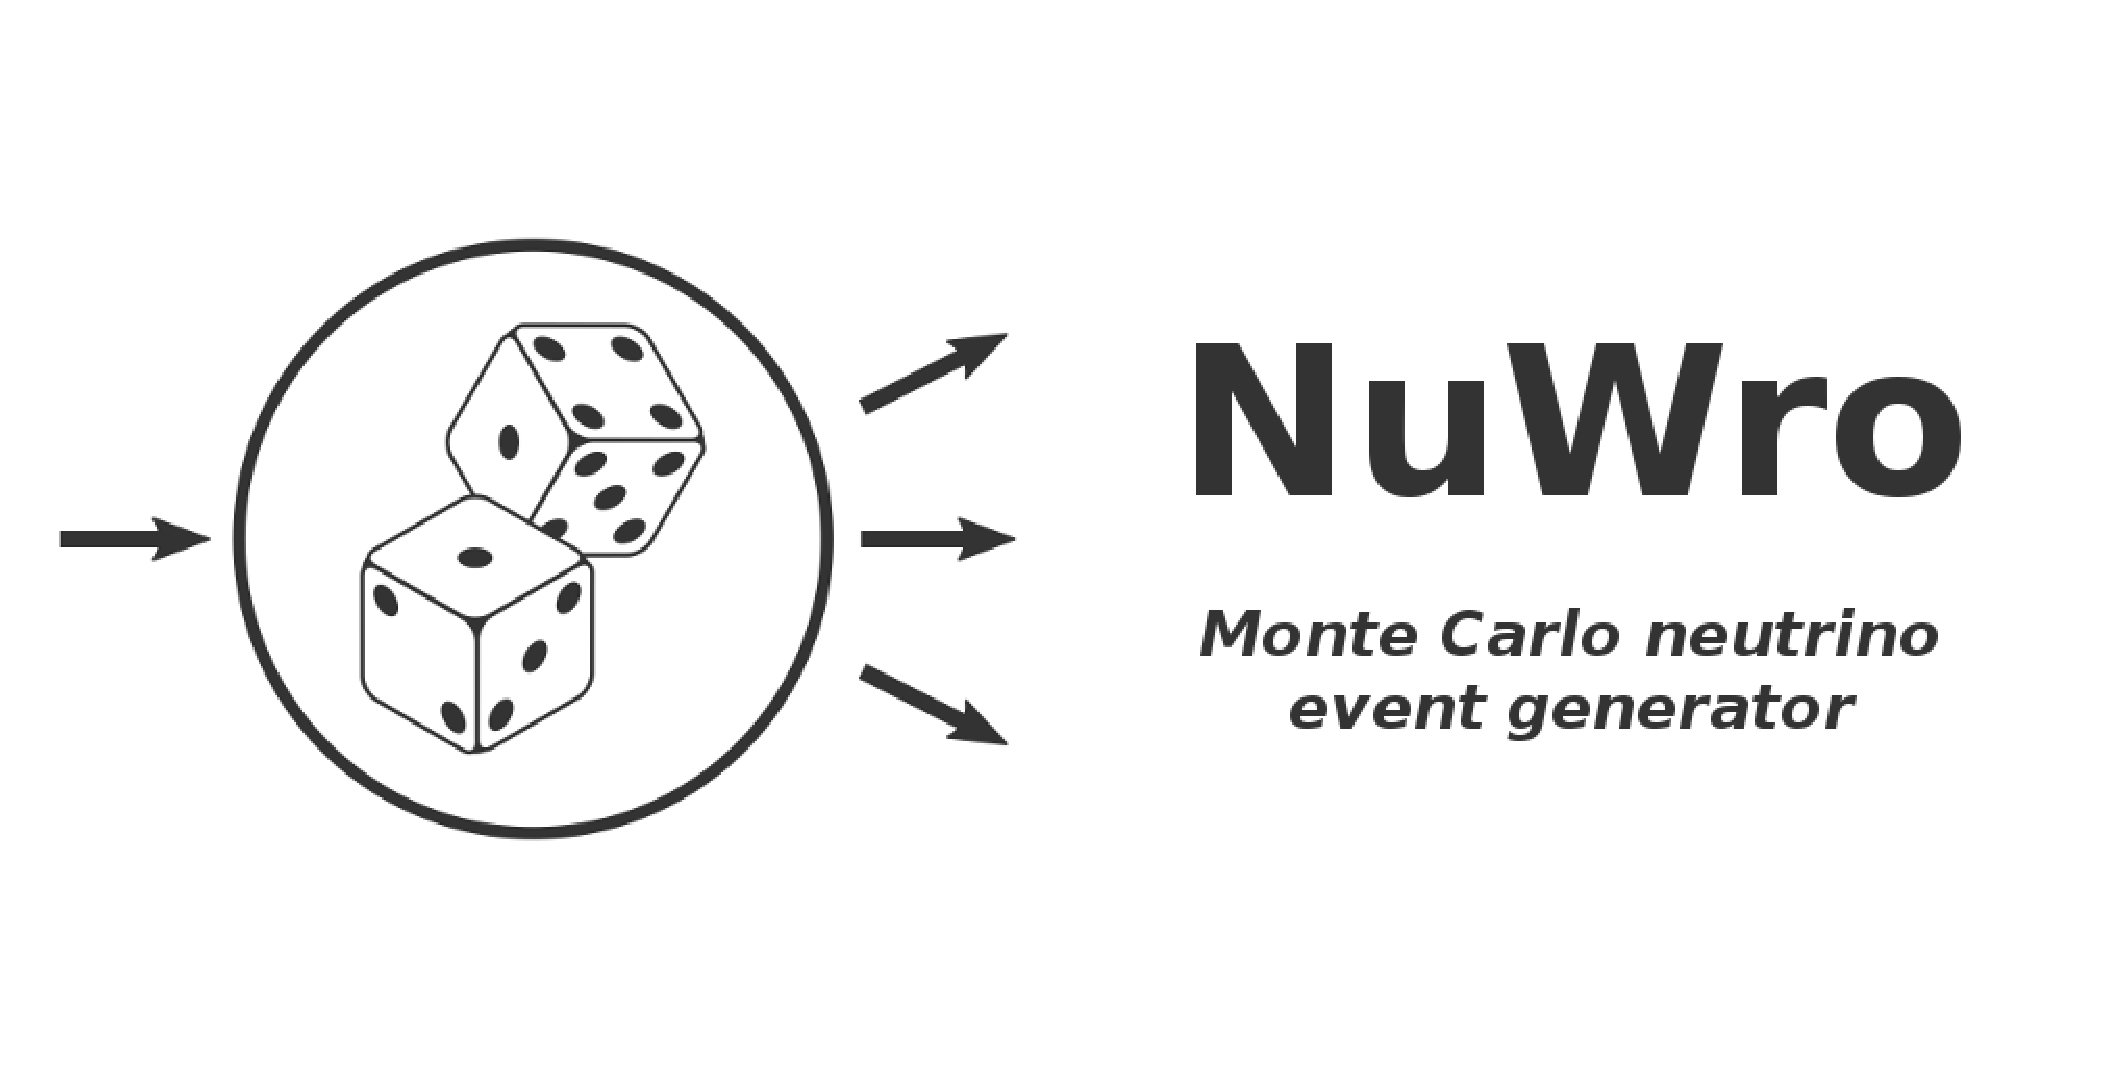
\includegraphics[width=0.75\columnwidth]{img/nuwro.eps}
  \end{center}
  \vspace{-30pt}
  {\it\hfill\grey{formerly known as WroNG}}
  
  \sep
  
  \begin{itemize}

    \item It has been developed at Wroclaw University since 2006
    \item The authors were encouraged by prof. Danuta Kie{\l}czewska from Warsaw University
    \item It is written in {\it\small C++} and uses {\it\small ROOT} library to store the output
    \item The open source code can be downloaded from the repository: \url{https://github.com/nuwro/}
%    \item (Local) Fermi Gas, as well as Spectral Function, can be used for the description of nucleons momenta.
%    \item Intranuclear cascade is available for nucleons and pions.
%    \item final state interactions are implemented.
%    \item Realistic beam models (eg T2K) and ability to use detector geometry read from a {\it\small ROOT} file (tested with T2K ND280 and MINERvA).
    
  \end{itemize}

\vfill\null
\end{slide}

%%%%% NuWro package %%%%%

\begin{emptyslide}[toc=]{}
\null\vfill

\centering\usetikzlibrary{mindmap,trees}

\tikzstyle{fullAngle}[1] = [level #1/.append style = {sibling angle = 360/\the\tikznumberofchildren}]
\tikzstyle{angle60}[1] = [level #1/.append style = {sibling angle = 60}]

\tikzset{level 1 concept/.append style = {font = \large, sibling angle = 90, level distance = 5cm, minimum size = 2.5cm}}
\tikzset{level 2 concept/.append style = {font = \normalsize, sibling angle = 60, level distance = 3.5cm, minimum size = 2cm}}
\tikzset{level 3 concept/.append style = {font = \small, sibling angle = 60, level distance = 3cm, minimum size = 2cm}}
\tikzset{level 4 concept/.append style = {font = \small, sibling angle = 60, level distance = 3cm, minimum size = 2cm}}

\scalebox{0.5}
{
\begin{tikzpicture}

  \path[mindmap, concept color = pdcolor1, text = pdcolor2]
  
  node[concept, minimum size = 1cm] {\Large\bf NuWro} [clockwise from = 90]
  child[concept color = pdcolor3!100!pdcolor1]
  {
    node[concept] {Interactions} [clockwise from = -150]
    child { node[concept] {QEL} }
    child { node[concept] {``RES''} }
    child { node[concept] {``DIS''} }
    child { node[concept] {MEC} }
    child { node[concept] {COH} }
  }  
  child[concept color = pdcolor5!100!pdcolor1]
  {
    node[concept] {Other} [clockwise from = 30]
    child {node[concept] {eWro} }
    child {node[concept] {NuWro on-line} }
  }
  child[concept color = pdcolor4!100!pdcolor1]
  {
    node[concept] {Nuclear Effects} [clockwise from = -30, level 2 concept/.append style = {sibling angle = 120}]
    child[concept]
    {
      node[concept] {Nucleus Model} [clockwise from = 30]
      child { node[concept] {Fermi Gas} }
      child { node[concept] {Spectral Function} }
    }
    child[concept]
    {
      node[concept] {FSI} [clockwise from = -150]
      child {node[concept] {Pions} }
      child { node[concept] {Nucleons} }
    }
  }
  child[concept color = pdcolor6!100!pdcolor1]
  { 
    node[concept] {Experiment} [clockwise from = -150]
    child {node[concept] {Beam} }
    child { node[concept] {Detector} }
  };

\end{tikzpicture}
}

\vfill\null
\end{emptyslide}

%%%% DYNAMICS %%%%%

\begin{wideslide}[toc=Dynamics]{Implemented dynamics}

  \rput(9.5,-3){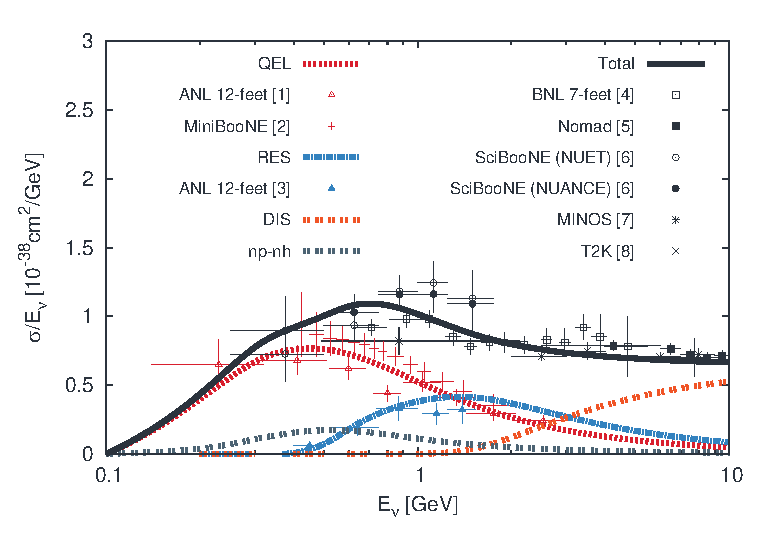
\includegraphics[width = 0.6\columnwidth]{img/xsec_cc2.eps}}

    
    \begin{itemize}
     \item All major interaction channels \\ are implemented, for charged and \\ neutral current, covering \\ neutrino energy region from \\ a few hundreds MeV \\ (Impulse Approximation limit) \\ to several TeV:
    \end{itemize}

%      \vspace{10pt}

      \begin{itemize}
	\addtolength{\itemindent}{10pt}
      
	\item[QEL] \red{(quasi-)elastic scattering}
	
	\item[RES] \blue{pion production through \\ \hspace{10pt}a $\Delta$ resonance excitation}
	
	\item[DIS] \orange{more inelastic processes}
	
	\item[COH] coherent pion production

	\item[np-nh] \grey{two body current contribution} %\\ \hspace{10pt}(Transverse Enhancement use on the plot).
      
      \end{itemize}

    \vspace{65pt}
    \rput[l](6.5,4.5){\color{pdcolor3}\footnotesize [1] PRD 19 (1979) 2521}
    \rput[l](6.5,4){\color{pdcolor3}\footnotesize [2] PRD 81 (2010) 092005}
    \rput[l](6.5,3.5){\color{pdcolor3}\footnotesize [3] PRD 16 (1977) 3103}
    \rput[l](6.5,3){\color{pdcolor3}\footnotesize [4] PRD 25 (1982) 617}
    \rput[l](10,4.5){\color{pdcolor3}\footnotesize [5] PLB 660 (2008) 19}
    \rput[l](10,4){\color{pdcolor3}\footnotesize [6] PRD 83 (2011) 012005}
    \rput[l](10,3.5){\color{pdcolor3}\footnotesize [7] PRD 81 (2011) 072002}
    \rput[l](10,3){\color{pdcolor3}\footnotesize [8] PRD 87 (2013) 092003}

\end{wideslide}

%%%%% QEL %%%%%%

\begin{slide}[toc=(Q)EL scattering]{(Quasi-)elastic scattering}
\null\vfill
  
  \twocolumn
  {
    \begin{itemize}
     \item Llewellyn-Smith model is used for charged current quasi-elastic scattering
     \item Not much difference here between generators (but default parameters)
    \end{itemize}
  }
  {
    \scalebox{0.75}{\begin{tikzpicture}[node distance = 1cm and 1.5cm]
  
 \node(left) [] {};
 \node(leftEmpty) [left=of left] {};
 \node(leftUp) [above=of leftEmpty] {$\nu / l$};
 \node(leftDown) [below=of leftEmpty] {$\nu$};
 
 \node(right) [right=of left] {};
 \node(rightEmpty) [right=of right] {};
 \node(rightUp) [above=of rightEmpty] {N'};
 \node(rightDown) [below=of rightEmpty] {N};
 
 \draw[curl, thick] (left.center) -- node[above] {$Z^0 / W^\pm$} ++ (right.center);
 
 \draw[color = pdcolor1, thick] (left.center) -- (leftUp);
 \draw[color = pdcolor1, thick] (left.center) -- (leftDown); 
 \draw[color = pdcolor1, thick] (right.center) -- (rightUp);
 \draw[color = pdcolor1, thick] (right.center) -- (rightDown);
 
\end{tikzpicture}
}
  }
  
  \sep
  
  \twocolumn
  {
    \centering\scalebox{0.5}{\begin{tikzpicture}
  
  \node (n) [circle, filled, minimum width = 4cm] {};

  \node (q1) [circle, filled={pdcolor5}, minimum width = 1cm, below=of n, yshift = 4.75cm] {}; 
  \node (q2) [circle, filled={pdcolor6}, minimum width = 1cm, below=of q1, xshift = 1cm] {}; 
  \node (q3) [circle, filled={pdcolor7}, minimum width = 1cm, below=of q1, xshift = -1cm] {};
 
  \draw [curl={pdcolor2}, very thick] (q1) -- (q2);
  \draw [curl={pdcolor2}, very thick] (q2) -- (q3);
  \draw [curl={pdcolor2}, very thick] (q3) -- (q1);

\end{tikzpicture}
}
  }
  {
    \sep
    \begin{itemize}
     \item Nucleon structure is parametrized by form factors
    \end{itemize}
  }

  \begin{itemize}
    \item Vector $\rightarrow$ Conserved Vector Current (CVC)
    \item Pseudo-scalar $\rightarrow$ Partially Conserved Axial Current (PCAC)
    \item Axial $\rightarrow$ dipole form with one free parameter (axial mass, $M_A$)
  \end{itemize}

  
\vfill\null
\end{slide}

%%%%% RES %%%%%

\begin{slide}[toc=RES pion production]{Resonance pion production}
\null\vfill

  \twocolumn
  {
    \begin{itemize}
      \item Most of generators (like NEUT and GENIE) uses Rein-Sehgal model
      \item RS model describes single pion production through baryon resonances below $W = 2$~GeV
    \end{itemize}
  }
  {
    \centering\scalebox{0.75}{\begin{tikzpicture}[node distance = 1cm and 1.5cm]
  
 \node(left) [] {};
 \node(leftEmpty) [left=of left] {};
 \node(leftUp) [above=of leftEmpty] {$\nu / l$};
 \node(leftDown) [below=of leftEmpty] {$\nu$};
 
 \node(right) [right=of left] {};
 \node(rightEmpty) [right=of right] {};
 \node(rightDown) [below=of rightEmpty] {N};

 \node(delta) [above=of rightEmpty, xshift = -1.0cm, yshift = -0.5cm] {$\Delta$};
 \node(rightUp1) [above=of delta, yshift = -0.5cm] {$\pi$};
 \node(rightUp2) [right=of delta, xshift = -1.0cm] {N'};
 
 \draw[curl, thick] (left.center) -- node[above] {$Z^0 / W^\pm$} ++ (right.center);
 
 \draw[color = pdcolor1, thick] (left.center) -- (leftUp);
 \draw[color = pdcolor1, thick] (left.center) -- (leftDown); 
 \draw[color = pdcolor1, thick] (right.center) -- (rightDown);
 \draw[color = pdcolor1, thick] (right.center) -- (delta);
 \draw[color = pdcolor1, thick] (delta) -- (rightUp1);
 \draw[color = pdcolor1, thick] (delta) -- (rightUp2);
 
\end{tikzpicture}
}
  }	

  \begin{itemize}
    \item In NuWro Adler-Rarita-Schwinger formalism is used to calculate $\Delta$ resonance explicitly
    \item Non-resonant background is estimated using quark-parton model
  \end{itemize}

\vfill\null
\end{slide}

%%%%% DIS %%%%%%

\begin{slide}[toc=Deep Inelastic Scattering]{Deep inelastic scattering [DIS]}
\null\vfill

  \twocolumn
  {
    \sep
    \begin{itemize}
     \item Quark-parton model is used for deep inelastic scattering
     \item Bodek-Young modification to the parton distributions at low $Q^2$ is included by most generators
    \end{itemize}
  }
  {
    \scalebox{0.75}{\begin{tikzpicture}[node distance = 1cm and 1.5cm]
  
 \node(left) [] {};
 \node(leftEmpty) [left=of left] {};
 \node(leftUp) [above=of leftEmpty] {$\nu / l$};
 \node(leftDown) [below=of leftEmpty] {$\nu$};
 
 \node(right) [right=of left] {};
 \node(rightEmpty) [right=of right] {};
 \node(rightDown) [below=of rightEmpty, xshift = -0.2cm, yshift = 0.2cm] {\scalebox{0.2}{\begin{tikzpicture}
  
  \node (n) [circle, filled, minimum width = 4cm] {};

  \node (q1) [circle, filled={pdcolor5}, minimum width = 1cm, below=of n, yshift = 4.75cm] {}; 
  \node (q2) [circle, filled={pdcolor6}, minimum width = 1cm, below=of q1, xshift = 1cm] {}; 
  \node (q3) [circle, filled={pdcolor7}, minimum width = 1cm, below=of q1, xshift = -1cm] {};
 
  \draw [curl={pdcolor2}, very thick] (q1) -- (q2);
  \draw [curl={pdcolor2}, very thick] (q2) -- (q3);
  \draw [curl={pdcolor2}, very thick] (q3) -- (q1);

\end{tikzpicture}
}};

 \node(rightUp) [above=of rightEmpty, xshift = -0.2cm, yshift = 0.2cm] {\scalebox{0.2}{\begin{tikzpicture}
  
  \node (center) {};
  
  \node [circle, filled={pdcolor4}, minimum width = 1cm, below=of center, xshift = 3cm, yshift = 0cm] {}; 
  \node [circle, filled={pdcolor5}, minimum width = 1cm, below=of center, xshift = 6cm, yshift = 1cm] {}; 
  \node [circle, filled={pdcolor6}, minimum width = 1cm, below=of center, xshift = 2cm, yshift = 2cm] {}; 
  \node [circle, filled={pdcolor7}, minimum width = 1cm, below=of center, xshift = 0cm, yshift = 3cm] {}; 
  \node [circle, filled={pdcolor4}, minimum width = 1cm, below=of center, xshift = 1cm, yshift = 4cm] {}; 
  \node [circle, filled={pdcolor5}, minimum width = 1cm, below=of center, xshift = 4cm, yshift = 3.5cm] {}; 
  \node [circle, filled={pdcolor6}, minimum width = 1cm, below=of center, xshift = 2.5cm, yshift = 3.5cm] {}; 
  \node [circle, filled={pdcolor7}, minimum width = 1cm, below=of center, xshift = 4.25cm, yshift = 1.5cm] {}; 
 
\end{tikzpicture}
}};
 
 \draw[curl, thick] (left.center) -- node[above] {$Z^0 / W^\pm$} ++ (right.center);
 
 \draw[color = pdcolor1, thick] (left.center) -- (leftUp);
 \draw[color = pdcolor1, thick] (left.center) -- (leftDown); 
 \draw[color = pdcolor1, thick, shorten >= -10pt] (right.center) -- (rightDown);

 \draw[color = pdcolor1, thick, shorten >= -10pt] (right.center) -- (rightUp);

\end{tikzpicture}
}
  }
  
  \myBoxFullWidth{Hadronization}
  
  \twocolumn
  {
    \sep\sep\sep
    \centering\scalebox{0.75}{\begin{tikzpicture}[node distance = 2cm]
  
  \node (quarks) {\scalebox{0.2}{\begin{tikzpicture}
  
  \node (center) {};
  
  \node [circle, filled={pdcolor4}, minimum width = 1cm, below=of center, xshift = 3cm, yshift = 0cm] {}; 
  \node [circle, filled={pdcolor5}, minimum width = 1cm, below=of center, xshift = 6cm, yshift = 1cm] {}; 
  \node [circle, filled={pdcolor6}, minimum width = 1cm, below=of center, xshift = 2cm, yshift = 2cm] {}; 
  \node [circle, filled={pdcolor7}, minimum width = 1cm, below=of center, xshift = 0cm, yshift = 3cm] {}; 
  \node [circle, filled={pdcolor4}, minimum width = 1cm, below=of center, xshift = 1cm, yshift = 4cm] {}; 
  \node [circle, filled={pdcolor5}, minimum width = 1cm, below=of center, xshift = 4cm, yshift = 3.5cm] {}; 
  \node [circle, filled={pdcolor6}, minimum width = 1cm, below=of center, xshift = 2.5cm, yshift = 3.5cm] {}; 
  \node [circle, filled={pdcolor7}, minimum width = 1cm, below=of center, xshift = 4.25cm, yshift = 1.5cm] {}; 
 
\end{tikzpicture}
}};
  \node (hadrons) [ell, notFilled, right=of quarks] {Hadrons};
  
  \draw [line, ->] (quarks) -- (hadrons);
 
\end{tikzpicture}
}
  }
  {
    \begin{itemize}
     \item Hadronization is the process of formation hadrons from quarks
     \item Pythia is widely used at high invariant masses
    \end{itemize}
  }

\vfill\null
\end{slide}

%%%%% RES / DIS %%%%%

\begin{slide}[toc=$\pi$ production]{Pion production in NuWro}
\null\vfill

  \centering\begin{tikzpicture}[node distance = 1.5cm and 1cm]
 
 \node(empty) {};
 
 \node(piprod) [rect, round, filled, above=of empty] {$\pi$ production};
 \node(delta)  [rect, notFilled, left=of empty, align = center] {$\Delta$ resonance \\ {\tiny Adler-Rarita-Schwinger}};
 \node(quark)  [rect, notFilled, right=of empty] {Quark-parton model};
 
 \node(res) [ell, filled, below=of delta] {RES};
 \node(dis) [ell, filled, below=of quark] {DIS};
 
 \draw [line, thick, ->] (piprod) -- (delta);
 \draw [line, thick, ->] (piprod) -- (quark);
 \draw [line, thick, ->] (delta) -- (res);

 \draw [line, thick, ->] (quark) -- node[above, rotate=25] {$W < 1.6$ GeV} ++ (res);
 \draw [line, thick, ->] (quark) -- node[right] {$W > 1.6$ GeV} ++ (dis);

 
\end{tikzpicture}


  \sep\sep
  
  \myFrameTextWidth[pdcolor6]{RES/DIS distinguish is arbitrary for each MC generator!}

\vfill\null
\end{slide}

%%%%% IMPULSE APPROXIMATION %%%%%

\begin{slide}{Impulse approximation}
\null\vfill

  \twocolumn
  {
    \begin{itemize}
      \item In impulse approximation neutrino interacts with a single nucleon
      \item If $|\vec q|$ is low the impact area usually includes many nucleons
      \item For high $|\vec q|$ IA is justified
    \end{itemize}    
  }
  {
    \centering\scalebox{0.5}{\begin{tikzpicture}
  
  \draw[ultra thick, color = pdcolor1] (0,0) circle (3);
  
  \node[circle,fill,color=pdcolor4,minimum size=0.75cm,text=white] at (0.253,-0.281) {$n$};
  \node[circle,fill,color=pdcolor4,minimum size=0.75cm,text=white] at (-1.83,0.434) {$n$};
  \node[circle,fill,color=pdcolor4,minimum size=0.75cm,text=white] at (-0.252,1.27) {$n$};
  \node[circle,fill,color=pdcolor4,minimum size=0.75cm,text=white] at (0.56,-1.52) {$n$};
  \node[circle,fill,color=pdcolor4,minimum size=0.75cm,text=white] at (-1.64,-0.932) {$n$};
  \node[circle,fill,color=pdcolor4,minimum size=0.75cm,text=white] at (1.93,0.932) {$n$};
  \node[circle,fill,color=pdcolor7,minimum size=0.75cm,text=white] at (0.843,0.684) {$p$};
  \node[circle,fill,color=pdcolor7,minimum size=0.75cm,text=white] at (-0.494,-1.67) {$p$};
  \node[circle,fill,color=pdcolor7,minimum size=0.75cm,text=white] at (1.48,-0.687) {$p$};
  \node[circle,fill,color=pdcolor7,minimum size=0.75cm,text=white] at (-1.2,1.64) {$p$};
  \node[circle,fill,color=pdcolor7,minimum size=0.75cm,text=white] at (-0.738,-0.163) {$p$};
  \node[circle,fill,color=pdcolor7,minimum size=0.75cm,text=white] at (0.561,2.03) {$p$};

  \draw[thick, color = pdcolor1] (-5,1) node[left] {$\nu$} -- (-4,-0.5) -- (-5, -2) node[left] {$\nu$};
  \draw[thick, color = pdcolor1, decorate, decoration = {coil,aspect=0,segment length=10pt,amplitude=3pt}] (-4,-0.5) -- (-0.9,-0.2);

\end{tikzpicture}}
  }
  
  \begin{itemize}
    \item Squares of transition matrices are summed up and interference terms are neglected
  
    $$\sigma^A = \sum\limits_{i = 1}^Z \sigma_p + \sum\limits_{i = 1}^{A - Z}\sigma_n$$
    
    \item High $|\vec q|$ means more than 400~MeV. However, IA is always assumed
  \end{itemize}
  
\vfill\null
\end{slide}

%%%%% FERMI GAS %%%%%%

\begin{slide}{Fermi gas}
\null\vfill

  \twocolumn
  {
    \myFrame{Nucleons move freely within the nuclear volume in constant binding potential.}
  }
  {
    \vspace*{-10pt}
    \scalebox{0.4}
{
\begin{tikzpicture}
     
  \draw[ultra thick, color=pdcolor1] (0,0) -- (3,0) -- (3, -4.7) -- (8,-4.7) -- (8,0) -- (11,0);
  \draw[ultra thick, dashed, color=pdcolor3] (0,0.1) to [out=0, in=210] (3, 1) to [out=30, in = 90](3.25, 0) -- (3.25, -3.7) -- (7.75, -3.7) -- (7.75, 0) to [out = 90, in = 150] (8,1) to [out = 330, in = 180] (11,0.1);
      
  \node[below, color=pdcolor1] at (4.3,0) {neutrons};
  \node[below, color=pdcolor3] at (6.8,0) {protons};
      
  \node[align = center, below, color=pdcolor1] at (1.5,-1.2) {neutrons \\ potential};
  \draw[thick,>=latex, ->, color=pdcolor1] (1.5,-1.2) -- (2,-0.1);
      
  \node[align = center, above, color=pdcolor3] at (9.5, 1.2) {protons \\ potential};
  \draw[thick,>=latex, ->, color=pdcolor3] (9.5,1.2) -- (9.2, 0.45);
      
  \draw[fill, color=pdcolor1] (3.8, -1.2) circle [radius=0.3];
  \draw[fill, color=pdcolor1] (4.8, -1.2) circle [radius=0.3];
  \draw[fill, color=pdcolor3] (6.2, -1.2) circle [radius=0.3];
  \draw[fill, color=pdcolor3] (7.2, -1.2) circle [radius=0.3];

  \draw[fill, color=pdcolor1] (3.8, -2.2) circle [radius=0.3];
  \draw[fill, color=pdcolor1] (4.8, -2.2) circle [radius=0.3];
  \draw[fill, color=pdcolor3] (6.2, -2.2) circle [radius=0.3];
  \draw[fill, color=pdcolor3] (7.2, -2.2) circle [radius=0.3];

  \draw[fill, color=pdcolor1] (3.8, -3.2) circle [radius=0.3];
  \draw[fill, color=pdcolor1] (4.8, -3.2) circle [radius=0.3];
  \draw[fill, color=pdcolor3] (6.2, -3.2) circle [radius=0.3];
  \draw[fill, color=pdcolor3] (7.2, -3.2) circle [radius=0.3];

  \draw[fill, color=pdcolor1] (3.8, -4.2) circle [radius=0.3];
  \draw[fill, color=pdcolor1] (4.8, -4.2) circle [radius=0.3];
      
  \draw[thick, dotted, color=pdcolor1] (8, -1.2) -- (11, -1.2);
  \draw[thick, dotted, color=pdcolor1] (8, -3.7) -- (9, -3.7);
  \draw[thick, dotted, color=pdcolor1] (8, -4.7) -- (11, -4.7);
      
  \draw[thick, >=latex, <->, color=pdcolor1] (8.5, -3.7) -- node[right]{$E_F^p$} (8.5, -1.2);
  \draw[thick, >=latex, <->, color=pdcolor1] (9.5, -4.7) -- node[right]{$E_F^n$} (9.5, -1.2);
  \draw[thick, >=latex, <->, color=pdcolor1] (10.5, -1.2) -- node[right]{$E_B$} (10.5, 0);
     
\end{tikzpicture}
}
  }
  \twocolumn
  {
    \myBox{Global Fermi Gas}
    $$p_F = \frac{\hbar}{r_0}\left(\frac{9\pi N}{4A}\right)^{1/3}$$  
  }
  {
    \myBox{Local Fermi Gas}
    $$p_F(r) = \hbar\left(3\pi^2\rho(r) \frac{N}{A}\right)^{1/3}$$  
  }
  
  \centering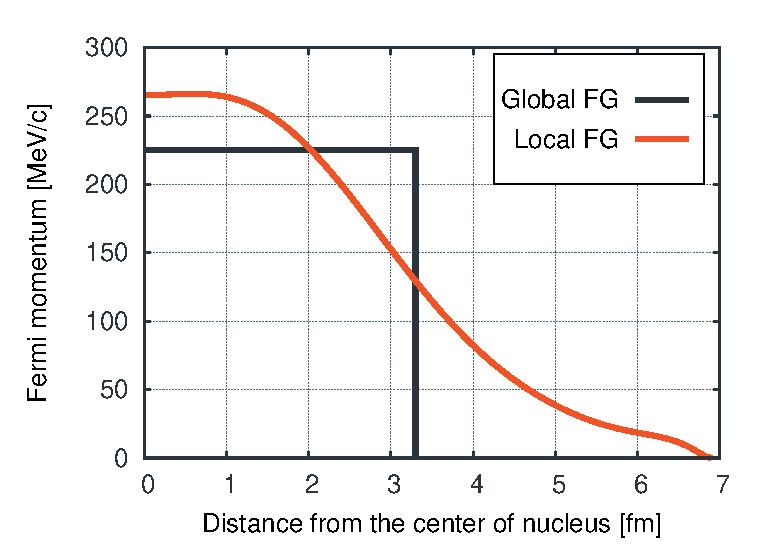
\includegraphics[width=0.5\columnwidth]{img/fermigas.eps}
  
\vfill\null
\end{slide}

%%%%% SPECTRAL FUNCTION %%%%%

\begin{wideslide}[toc=Spectral function]{Spectral function}
\null\vfill
    
  \twocolumn
  {
    \sep\sep
    \myFrame{The probability of removing of a nucleon with momentum $\vec p$ and leaving residual nucleus with excitation energy $E$.}
    $$P (\vec p, E) = P_{MF} (\vec p, E) + P_{corr} (\vec p, E)$$
    \rput[c](7.5, 2.0){\scalebox{0.75}{\begin{pspicture}
   
  \psline[linewidth = 0.025, linecolor = pdcolor6, doubleline]{<->}(-0.9,0)(-0.6,-0.75)
  
  \psline[linewidth = 0.1, linecolor = pdcolor3]{->}(-0.5,-1)(-0.2, -1.75)
  \psline[linewidth = 0.1, linecolor = pdcolor3]{->}(-1,0.25)(-1.3, 1)
   
  \pscircle[linewidth = 0.05, linecolor = pdcolor1](0,0){2}
  \pscircle[linestyle = none, fillstyle = solid, fillcolor = pdcolor1](0.75,1){0.2}
  \pscircle[linestyle = none, fillstyle = solid, fillcolor = pdcolor1](-0.5,1.25){0.2}
  \pscircle[linestyle = none, fillstyle = solid, fillcolor = pdcolor1](-1,0.25){0.2}
  \pscircle[linestyle = none, fillstyle = solid, fillcolor = pdcolor1](0,0.25){0.2}
  %\pscircle[linestyle = none, fillstyle = solid, fillcolor = pdcolor1](0.6, -0.75){0.2}
  \pscircle[linestyle = none, fillstyle = solid, fillcolor = pdcolor4](-0.5, -1){0.2}
  \pscircle[linestyle = none, fillstyle = solid, fillcolor = pdcolor1](1.25, 0){0.2}
  
  \pscoil[coilarm = 0, linewidth = 0.025, linecolor = pdcolor1, coilwidth = 0.15, coilaspect = 0]{c-c}(-2.5,0)(-1,0.25)
  \psline[linewidth = 0.025, linecolor = pdcolor1]{-c}(-3.5, -1)(-2.5,0)
  \psline[linewidth = 0.025, linecolor = pdcolor1]{-c}(-3.5, 1)(-2.5,0)
  \rput[l](-3.5,1.2){\color{pdcolor1} $l'$}
  \rput[l](-3.5,-1.2){\color{pdcolor1} $l$}
  \rput[c](0.5, -1){\color{pdcolor4} spectator}
  \rput[c]{-66}(-0.53, -0.23){\color{pdcolor6} SRC}
     
\end{pspicture}
}}
  }
  {
    \vspace*{-10pt}
    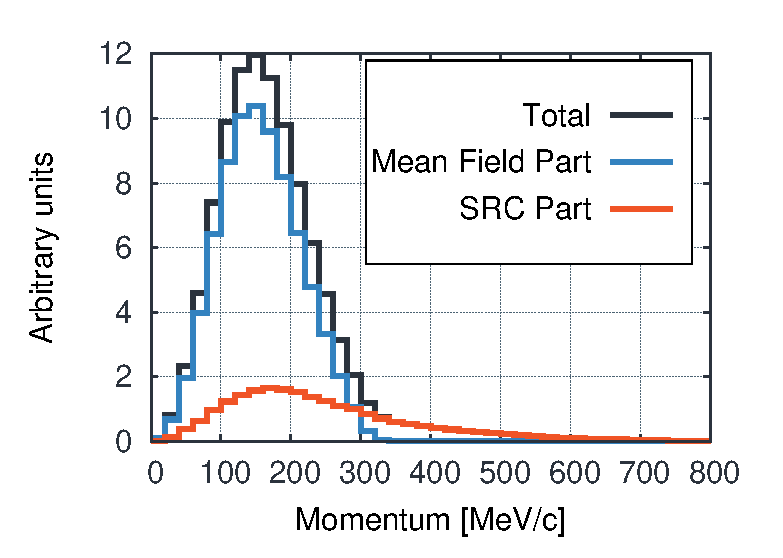
\includegraphics[width=\columnwidth]{img/sf_mom.eps}
    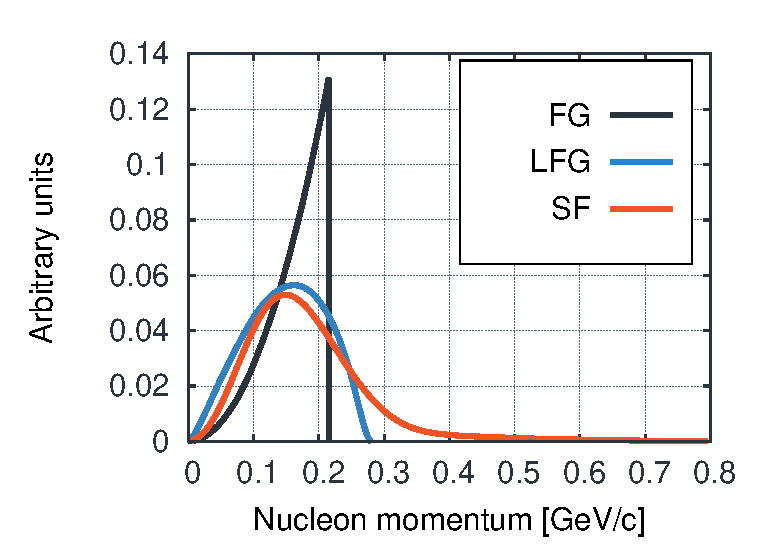
\includegraphics[width=\columnwidth]{img/fg_vs_sf.eps}  
  }

\vfill\null
\end{wideslide}

%%%%% TWO-BODY %%%%%

\begin{slide}[toc=Two-body current]{Two-body current interactions}
\null\vfill

  \sep
  \twocolumn
  {
    \begin{tikzpicture}[node distance = 0.5cm and 0.5cm]
 
  \node(tbc)  [rect, round, notFilled, minimum width = 5cm, text width = 5cm] {Two Body Current};
  \node(2p2h) [rect, round, notFilled, below=of tbc, minimum width = 5cm, text width = 5cm] {2 particles - 2 holes (2p-2h)};
  \node(mec)  [rect, round, notFilled, below=of 2p2h, minimum width = 5cm, text width = 5cm] {Meson Exchange Current (MEC)};
   
\end{tikzpicture}

  }
  {
    \rput[c](6.5, 1.6){\scalebox{0.75}{\begin{pspicture}
   
  \psline[linewidth = 0.025, linecolor = pdcolor6, linestyle=dashed]{-}(-1,0.2)(-0.55,-0.85)
  
  \psline[linewidth = 0.1, linecolor = pdcolor3]{->}(-0.5,-1)(-0.2, -1.75)
  \psline[linewidth = 0.1, linecolor = pdcolor3]{->}(-1,0.25)(-1.3, 1)
   
  \pscircle[linewidth = 0.05, linecolor = pdcolor1](0,0){2}
  \pscircle[linestyle = none, fillstyle = solid, fillcolor = pdcolor1](0.75,1){0.2}
  \pscircle[linestyle = none, fillstyle = solid, fillcolor = pdcolor1](-0.5,1.25){0.2}
  \pscircle[linestyle = none, fillstyle = solid, fillcolor = pdcolor1](-1,0.25){0.2}
  \pscircle[linestyle = none, fillstyle = solid, fillcolor = pdcolor1](0,0.25){0.2}
  %\pscircle[linestyle = none, fillstyle = solid, fillcolor = pdcolor1](0.6, -0.75){0.2}
  \pscircle[linestyle = none, fillstyle = solid, fillcolor = pdcolor1](-0.5, -1){0.2}
  \pscircle[linestyle = none, fillstyle = solid, fillcolor = pdcolor1](1.25, 0){0.2}
  
  \pscoil[coilarm = 0, linewidth = 0.025, linecolor = pdcolor1, coilwidth = 0.15, coilaspect = 0]{c-c}(-2.5,0)(-0.9,-0.35)
  \psline[linewidth = 0.025, linecolor = pdcolor1]{-c}(-3.5, -1)(-2.5,0)
  \psline[linewidth = 0.025, linecolor = pdcolor1]{-c}(-3.5, 1)(-2.5,0)
  
  \rput[l](-3.5,1.2){\color{pdcolor1} $l'$}
  \rput[l](-3.5,-1.2){\color{pdcolor1} $l$}
  \rput[c]{-66}(-0.53, -0.23){\color{pdcolor6} VM}
     
\end{pspicture}
}}
  }
  
  \vspace{-20pt}
  
  \myBoxFullWidth{Models in generators}
  
  \begin{itemize}
    \item Nieves model (GENIE, NEUT, NuWro) - CC only
    \item Transverse Enhancement model (NuWro) - both CC and NC
  \end{itemize}
  
\vfill\null
\end{slide}

\begin{wideslide}[toc=]{Two-body current interactions}
\null\vfill

  \begin{itemize}
    \item Nieves model is microscopic calculation
    \item TE model introduce $2p-2h$ contribution by modification of the vector magnetic form factors
  \end{itemize}
  
  \sep\sep

  \twocolumn
  {
    \myBox{Total MEC cross section}
    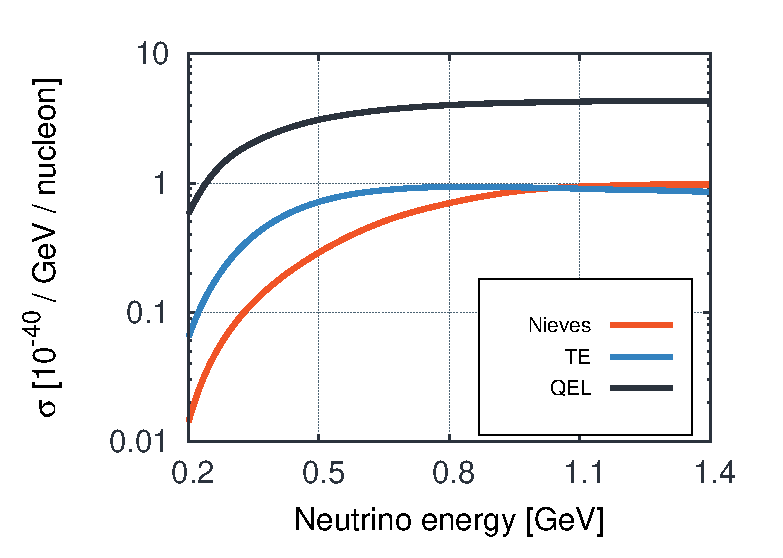
\includegraphics[width=\columnwidth]{img/mec_xsec.eps}
  }
  {
    \myBox{MEC / (QEL + MEC)}
    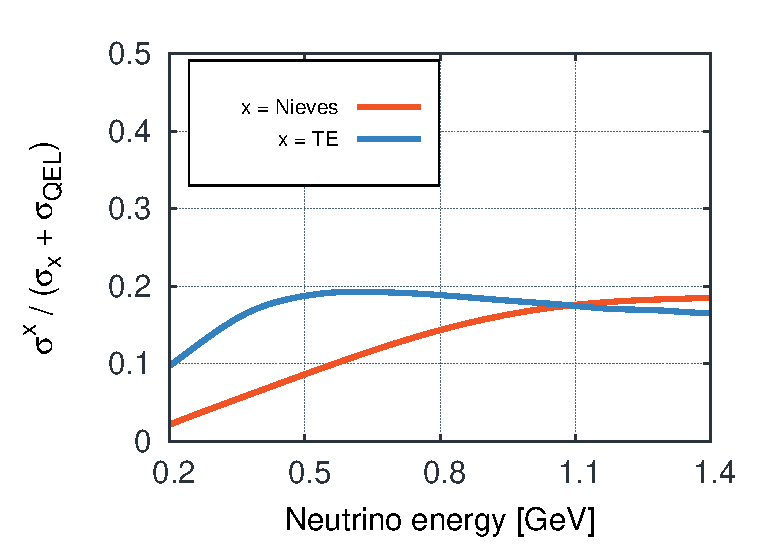
\includegraphics[width=\columnwidth]{img/mec_ratio.eps}  
  }


\vfill\null
\end{wideslide}

\begin{wideslide}[toc=]{Two-body current interactions}
\null\vfill

  \begin{itemize}
    \item Both models provide only the inclusive double differential cross section for the final state lepton
    \item Final nucleons momenta are set isotropically in CMS
  \end{itemize}

  \sep\sep
  
  \twocolumn
  {
    \myBox{Nieves}
    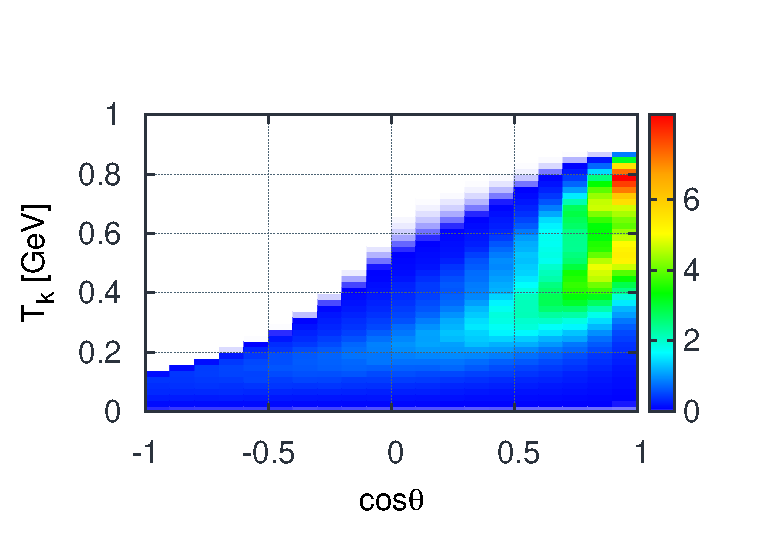
\includegraphics[width=\columnwidth]{img/mec_lep_nieves.eps}
  }
  {
    \myBox{Transverse Enhancement}
    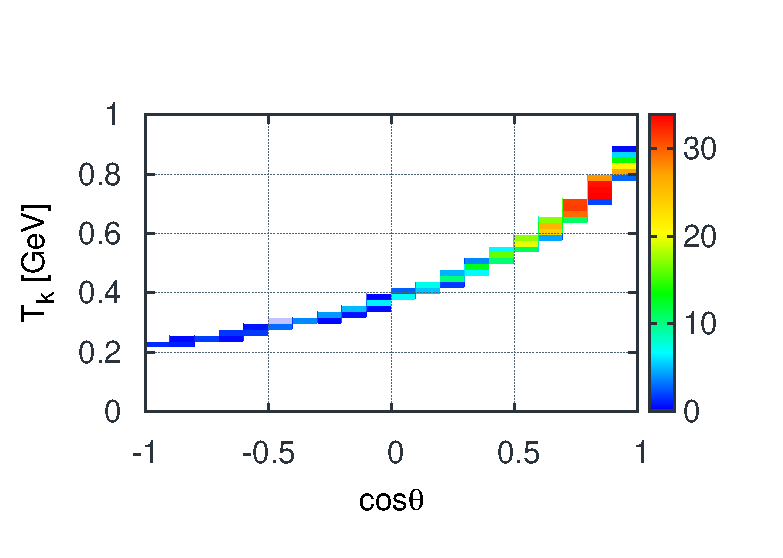
\includegraphics[width=\columnwidth]{img/mec_lep_tem.eps}
  }


\vfill\null
\end{wideslide}

%%%%% COHERENT PION PRODUCTION %%%%%

\begin{slide}[toc=COH pion production]{Coherent pion production}
\null\vfill

  \twocolumn
  {
    \begin{itemize}
      \item Rein-Sehgal model is commonly used for coherent pion production
      \item Note: it is different model than for RES
      \item Berger-Sehgal model replaces RS (NuWro, GENIE - coming soon)
    \end{itemize}
  }
  {
    \sep\sep
    \scalebox{0.75}{\begin{tikzpicture}[node distance = 1cm and 1.5cm]
  
 \node(left) [] {};
 \node(leftEmpty) [left=of left] {};
 \node(leftUp) [above=of leftEmpty] {$\nu / l$};
 \node(leftDown) [below=of leftEmpty] {$\nu$};
 
 \node(right) [right=of left] {};
 \node(rightEmpty) [right=of right] {};
 \node(rightUp) [above=of rightEmpty] {$\pi$};
 
 \node(A) [below=of right, xshift = -1cm, yshift = 0.2cm, circle, notFilled, text width = 0.75cm] {A,Z};
 \node(Aprim) [below=of right, xshift =  1cm, yshift = 0.2cm, circle, notFilled, text width = 0.75cm] {A,Z};
 
 \draw[curl, thick] (left.center) -- node[above] {$Z^0 / W^\pm$} ++ (right.center);
 
 \draw[color = pdcolor1, thick] (left.center) -- (leftUp);
 \draw[color = pdcolor1, thick] (left.center) -- (leftDown); 
 \draw[color = pdcolor1, thick] (right.center) -- (rightUp);
 \draw[color = pdcolor1, very thick, ->] (A) -- (Aprim);
 \draw[color = pdcolor1, thick, dashed, double] (right) -- ([xshift = 1cm]A.center);
 
\end{tikzpicture}
}
  }
  
  \vspace*{-10pt}
  
  \myBoxFullWidth[pdcolor3]{Comments}
  
  \begin{itemize}
    \item In COH the residual nucleus is left in the same state (not excited)
    \item The interaction occurs on a whole nucleus - no final state interactions
  \end{itemize}

\vfill\null
\end{slide}

%%%%% INTERACTIONS SUMMARY %%%%%%

\begin{slide}[toc=Summary]{Neutrino interactions - summary}
\null\vfill

  \begin{tikzpicture}[node distance = 1cm and 1cm]
 
 \node(nucleon) [notFilled={pdcolor1}, rect]                   {Nucleon (IA*)};
 \node(npnh) 	[notFilled={pdcolor1}, rect, right=of nucleon] {np-nh (semi-IA)};
 \node(nucleus) [notFilled={pdcolor1}, rect, right=of npnh]    {Nucleus};
 
 \node(neutrino) [filled={pdcolor1}, rect, round, above=of npnh] {Neutrino};
 
 \draw[line={pdcolor1}, ultra thick, ->] (neutrino.south west) -- (nucleon.north east);
 \draw[line={pdcolor1}, ultra thick, ->] (neutrino.south)      -- (npnh.north);
 \draw[line={pdcolor1}, ultra thick, ->] (neutrino.south east) -- (nucleus.north west);
 
 \begin{scope}[node distance = 0.5cm]
  \node(qel) [filled={pdcolor3}, ell, below=of nucleon] {(Q)EL};  
  \node(res) [filled={pdcolor3}, ell, below=of qel]     {RES};  
  \node(dis) [filled={pdcolor3}, ell, below=of res]     {DIS};
  \node(mec) [filled={pdcolor3}, ell, below=of npnh]    {MEC (2p2h)};
  \node(coh) [filled={pdcolor3}, ell, below=of nucleus] {Coherent $\pi$};
 \end{scope}

 \node(fsi) [filled={pdcolor4}, rect, round, minimum width = 5cm, text width = 5cm, right=of dis, xshift=0.5cm, yshift=0.75cm] {Final state interactions};
 
 \draw[line={pdcolor3}, thick, ->] (qel.south east) -- (fsi.north west);
 \draw[line={pdcolor3}, thick, ->] ([xshift=-3pt, yshift=-5pt] res.east) -- (fsi.west);
 \draw[line={pdcolor3}, thick, ->] (dis.east)       -- (fsi.south west);
 \draw[line={pdcolor3}, thick, ->] (mec.south)      -- ([xshift=-1.75cm]fsi.north);
 
 \node [below=of fsi, xshift = 2cm] {*IA = Impulse Approximation};
 
\end{tikzpicture}



\vfill\null
\end{slide}


\end{document}
